\documentclass[usenames,dvipsnames,11pt,pdf,utf8,russian,aspectratio=169]{beamer}
\usepackage{cmap}
%\usepackage[T2A]{fontenc}
%\usepackage[english,russian]{babel}
\usepackage{subfig}
\usepackage{color}
\usepackage{multicol}
\usepackage{appendixnumberbeamer}
\usepackage{multicol}
\usepackage{tikz}
\usepackage{mathbbol}
\usepackage{amsmath}   
\usepackage{amssymb}   
\usepackage{xargs}             % AMS Math

\DeclareFontShape{OT1}{cmss}{b}{n}{<->ssub * cmss/bx/n}{} %https://tex.stackexchange.com/questions/565069/beamer-bold-math-no-longer-working


\DeclareUnicodeCharacter{00A0}{ } % При наборе текста с планшета появляются невидимые символы. ЭТо костыль.

\DeclareSymbolFontAlphabet{\mathbb}{AMSb}%
\DeclareSymbolFontAlphabet{\amsmathbb}{bbold}%


\usetikzlibrary{arrows,automata}
\usetikzlibrary{positioning}



\DeclareMathOperator*{\argmin}{arg\,min}

\DeclareMathOperator*{\argmax}{arg\,max}
%
% Choose how your presentation looks.
%
% For more themes, color themes and font themes, see:
% http://deic.uab.es/~iblanes/beamer_gallery/index_by_theme.html
%
\mode<presentation>
{
  \usetheme{Boadilla}      % or try Darmstadt, Madrid, Warsaw, ...
  \usecolortheme{seagull} % or try albatross, beaver, crane, ..

  \usefonttheme{structurebold}  % or try serif, structurebold, ...
  \setbeamertemplate{navigation symbols}{}
  \setbeamertemplate{caption}[numbered]

} 
\setbeamercolor{mygray}{fg=gray,bg=white}


\setbeamertemplate{footline}
{
  \leavevmode%
  \hbox{%
  \begin{beamercolorbox}[wd=.9\paperwidth,ht=2.25ex,dp=1ex,center]{}%
   
  \end{beamercolorbox}%
  \begin{beamercolorbox}[wd=.1\paperwidth,ht=2.25ex,dp=1ex]{mygray}%
   
    \insertframenumber{} / \inserttotalframenumber\hspace*{1ex}
  \end{beamercolorbox}}%
  \vskip0pt%
}



\captionsetup[subfloat]{labelformat=empty}
\title[Model structure selection]{Bayesian selection of \\deep learning model structure}
\author{Oleg Bakhteev, Vadim Strijov}



%\institute[МФТИ]{Московский Физико-Технический Институт (Государственный Университет)}
\date[2021]{Moscow Institute of Physics and Technology\\July 2, 2021}
\begin{document}
% nb: очень не люблю макросы. Но что поделать 
% https://stackoverflow.com/questions/1509799/how-to-replace-latex-macros-with-their-definitions-using-latex
\newcommand{\D}{\mathfrak{D}}
\newcommand{\x}{\mathbf{x}}
\newcommand{\X}{\mathbf{X}}
\newcommand{\y}{\mathbf{y}}
\newcommand{\Xb}{\mathbb{X}}
\newcommand{\yb}{\mathbb{Y}}
\newcommand{\F}{\mathfrak{F}}



\newcommand{\w}{\mathbf{w}}
\newcommand{\Wb}{\mathbb{W}}
\newcommand{\Uw}{U_\mathbf{w}}

\newcommand{\Gam}{\boldsymbol{\Gamma}}
\newcommand{\Gb}{\amsmathbb{\Gamma}}
\newcommand{\UG}{U_{\boldsymbol{\Gamma}}}

\newcommand{\h}{\mathbf{h}}
\newcommand{\Hb}{\mathbb{H}}
\newcommand{\Uh}{U_{\mathbf{h}}}

\newcommand{\teta}{\boldsymbol{\theta}}
\newcommand{\Tetab}{\amsmathbb{\Theta}}
\newcommand{\Uteta}{U_{\boldsymbol{\theta}}}

\newcommand{\tetaw}{\boldsymbol{\theta}_\mathbf{w}}
\newcommand{\Tetawb}{\amsmathbb{\Theta}_\mathbf{w}}
\newcommand{\Utetaw}{U_{\boldsymbol{\theta}_\mathbf{w}}}
\newcommand{\tetaG}{\boldsymbol{\theta}_{\boldsymbol{\Gamma}}}
\newcommand{\TetaGb}{\amsmathbb{\Theta}_{\boldsymbol{\Gamma}}}
\newcommand{\UtetaG}{U_{\boldsymbol{\theta}_{\boldsymbol{\Gamma}}}}

\newcommand{\lam}{\boldsymbol{\lambda}}
\newcommand{\Lamb}{\amsmathbb{\Lambda}}
\newcommand{\Ulam}{U_{\boldsymbol{\lambda}}}

%\newcommand{\prior}{p(\mathbf{w}, \boldsymbol{\Gamma}|\mathbf{h},\boldsymbol{\lambda})}
\newcommandx{\prior}[4][1=\mathbf{w},2=\boldsymbol{\Gamma},3=\mathbf{h},4=\boldsymbol{\lambda},usedefault]{p(#1,#2|#3,#4)}
\newcommandx{\priorh}[2][1=\mathbf{h}, 2=\boldsymbol{\lambda},usedefault]{p(#1|#2)}
\newcommandx{\priorG}[3][1=\boldsymbol{\Gamma}, 2= \mathbf{h}, 3=\boldsymbol{\lambda},usedefault]{p(#1|#2,#3)}
\newcommandx{\priorw}[4][1=\mathbf{w},2=\boldsymbol{\Gamma},3=\mathbf{h},4=\boldsymbol{\lambda},usedefault]{p(#1|#2,#3,#4)}


\newcommand{\post}{p(\mathbf{w}, \boldsymbol{\Gamma}|\mathbf{y}, \mathbf{X}, \mathbf{h},\boldsymbol{\lambda})}
\newcommand{\posth}{p(\mathbf{h}|\mathbf{y}, \mathbf{X},\boldsymbol{\lambda})}
\newcommand{\postG}{p(\boldsymbol{\Gamma}|\mathbf{y}, \mathbf{X}, \mathbf{h},\boldsymbol{\lambda})}
\newcommand{\postw}{p(\mathbf{w}|\mathbf{y}, \mathbf{X}, \boldsymbol{\Gamma}, \mathbf{h},\boldsymbol{\lambda})}


\newcommandx{\q}[1][1=\boldsymbol{\theta}, usedefault]{q(\mathbf{w}, \boldsymbol{\Gamma}|#1)}
\newcommandx{\qG}[2][1=\boldsymbol{\Gamma},2=\boldsymbol{\theta}_{\boldsymbol{\Gamma}},usedefault]{q_{\boldsymbol{\Gamma}}(#1|#2)}
\newcommandx{\qw}[3][1=\mathbf{w}, 2=\boldsymbol{\Gamma},3=\boldsymbol{\theta}_\mathbf{w},usedefault]{q_\mathbf{w}(#1|#2,#3)}


\newcommandx{\LL}[4][1=\mathbf{y},2=\mathbf{X},3=\mathbf{w},4=\boldsymbol{\Gamma},usedefault]{p(#1|#2,#3,#4)}

\newcommand{\EV}{p(\mathbf{y}|\mathbf{X}, \mathbf{h},\boldsymbol{\lambda})}

\newcommandx{\Loss}[5][1=\boldsymbol{\theta},2=\mathbf{y},3=\mathbf{X},4=\mathbf{h},5=\boldsymbol{\lambda},usedefault]{L(#1 |#2,#3,#4,#5)}
\newcommandx{\Val}[5][1=\mathbf{h},2=\mathbf{y},3=\mathbf{X},4=\boldsymbol{\theta},5=\boldsymbol{\lambda},usedefault]{Q(#1|#2,#3,#4,#5)}

% прочее
\newcommand{\model}{\mathbf{f}}
\newcommand{\A}{\mathbf{A}}
\newcommand{\s}{\mathbf{s}}
\newcommand{\g}{\boldsymbol{\gamma}}
\newcommand{\E}{\mathsf{E}}
\newcommand{\KL}[2]{D_\text{KL}\bigl(#1 || #2\bigr)}

\newcommand{\lamT}{\lambda_{\text{temp}}}
\newcommand{\lamLL}{\lambda_\text{likelihood}^\text{Q}}
\newcommand{\lamCL}{\lambda_\text{prior}^\text{L}}
\newcommand{\lamCQ}{\lambda_\text{prior}^\text{Q}}
\newcommand{\lamS}{\boldsymbol{\lambda}_\text{struct}^\text{Q}}
\newcommandx{\TLoss}[6][1=\boldsymbol{\theta},2=L,3=\mathbf{y}, 4=\mathbf{X}, 5=\mathbf{h},6=\boldsymbol{\lambda},usedefault]{T(#1|#2,#3,#4,#5,#6)}
\newcommandx{\TVal}[6][1=\mathbf{h},2=Q,3=\mathbf{y}, 4=\mathbf{X}, 5=\boldsymbol{\teta},6=\boldsymbol{\lambda},usedefault]{T(#1|#2,#3,#4,#5,#6)}
%\newcommand{\log}{\text{log}~}




\begin{frame}
  \titlepage
\end{frame}





\begin{frame}    
                                                                                                                        
\frametitle{Model structure selection challenge}     
Data likelihood does not change with removing redundant parameters.
\begin{figure}[h]                                                                                                                               
\centering                                                                                                                                      
\subfloat[Redundancy of model parameters]{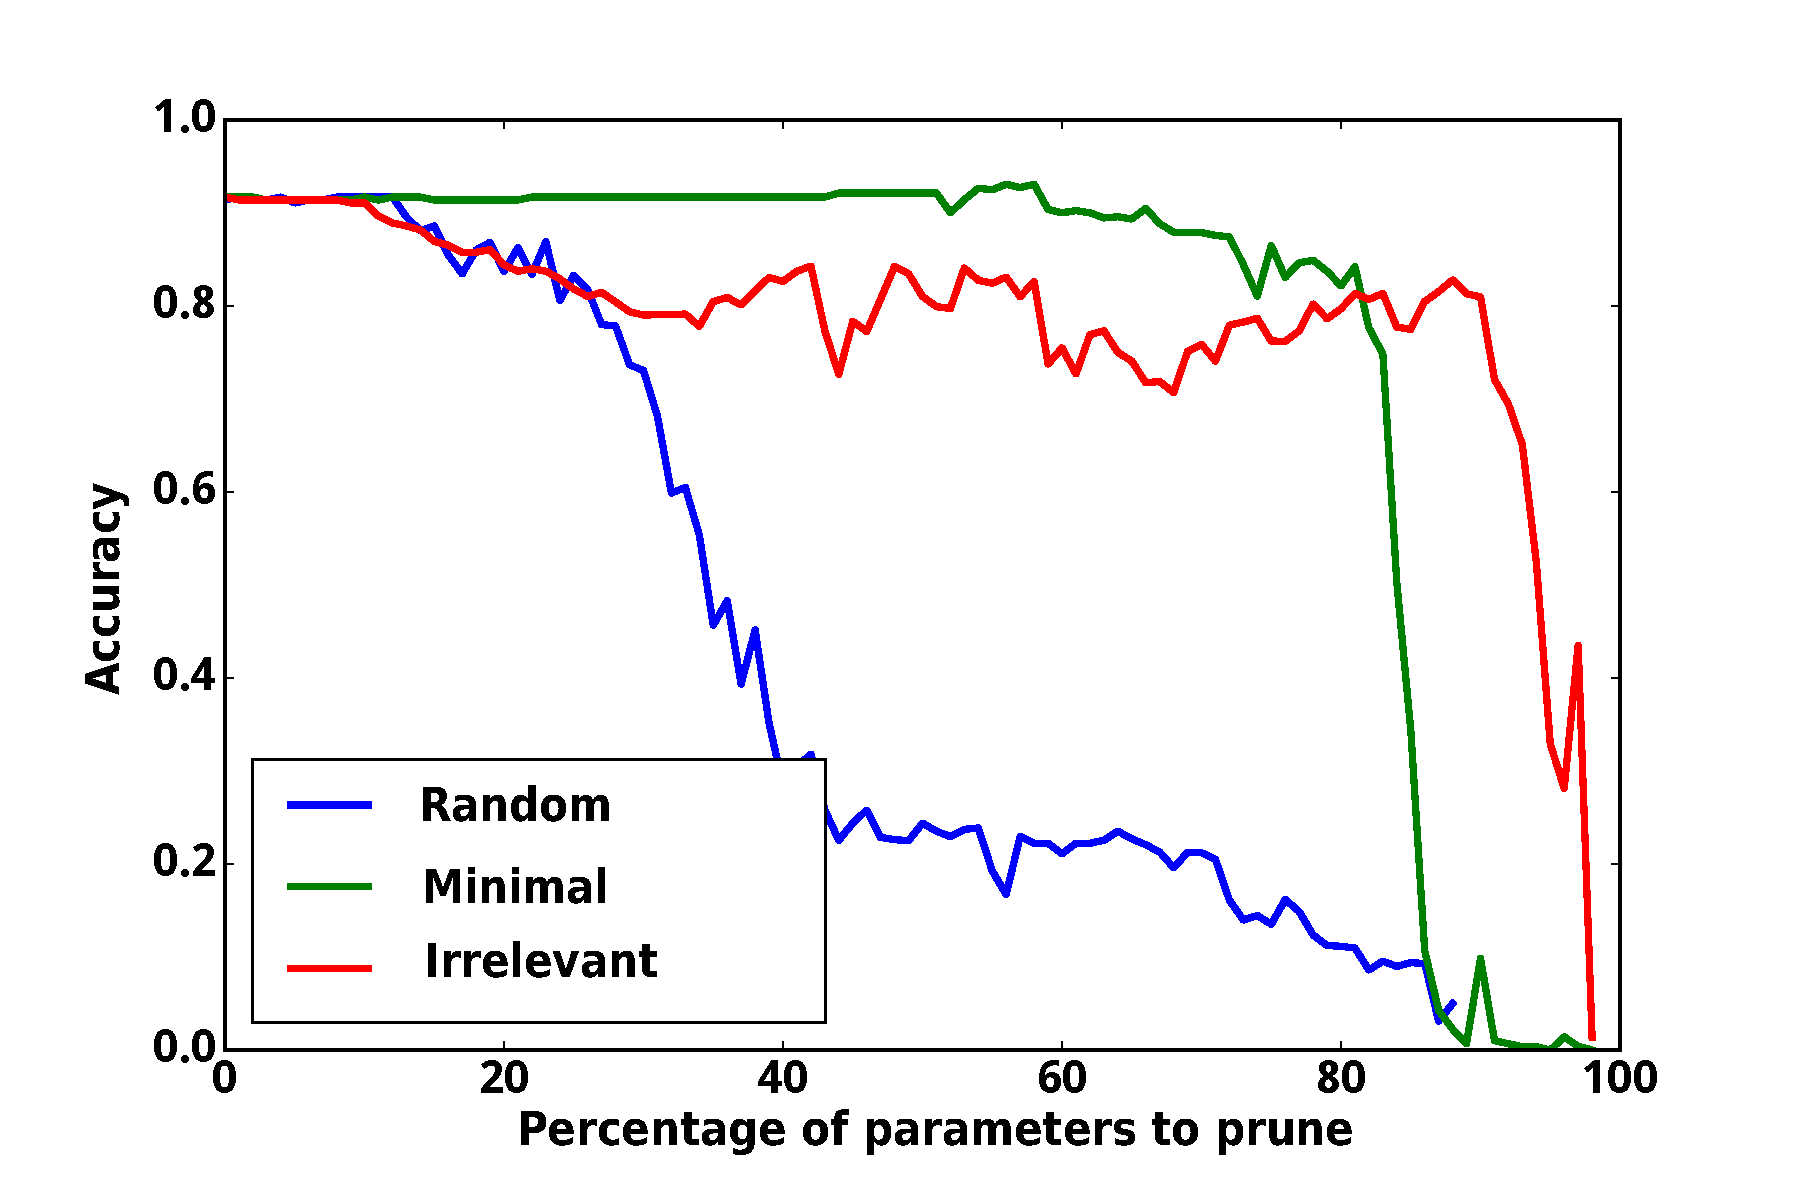
\includegraphics[width=0.55\textwidth]{./slide_plots/pruning_eng.pdf}}   
\hspace*{-1cm}                                       
\subfloat[Model robustness]{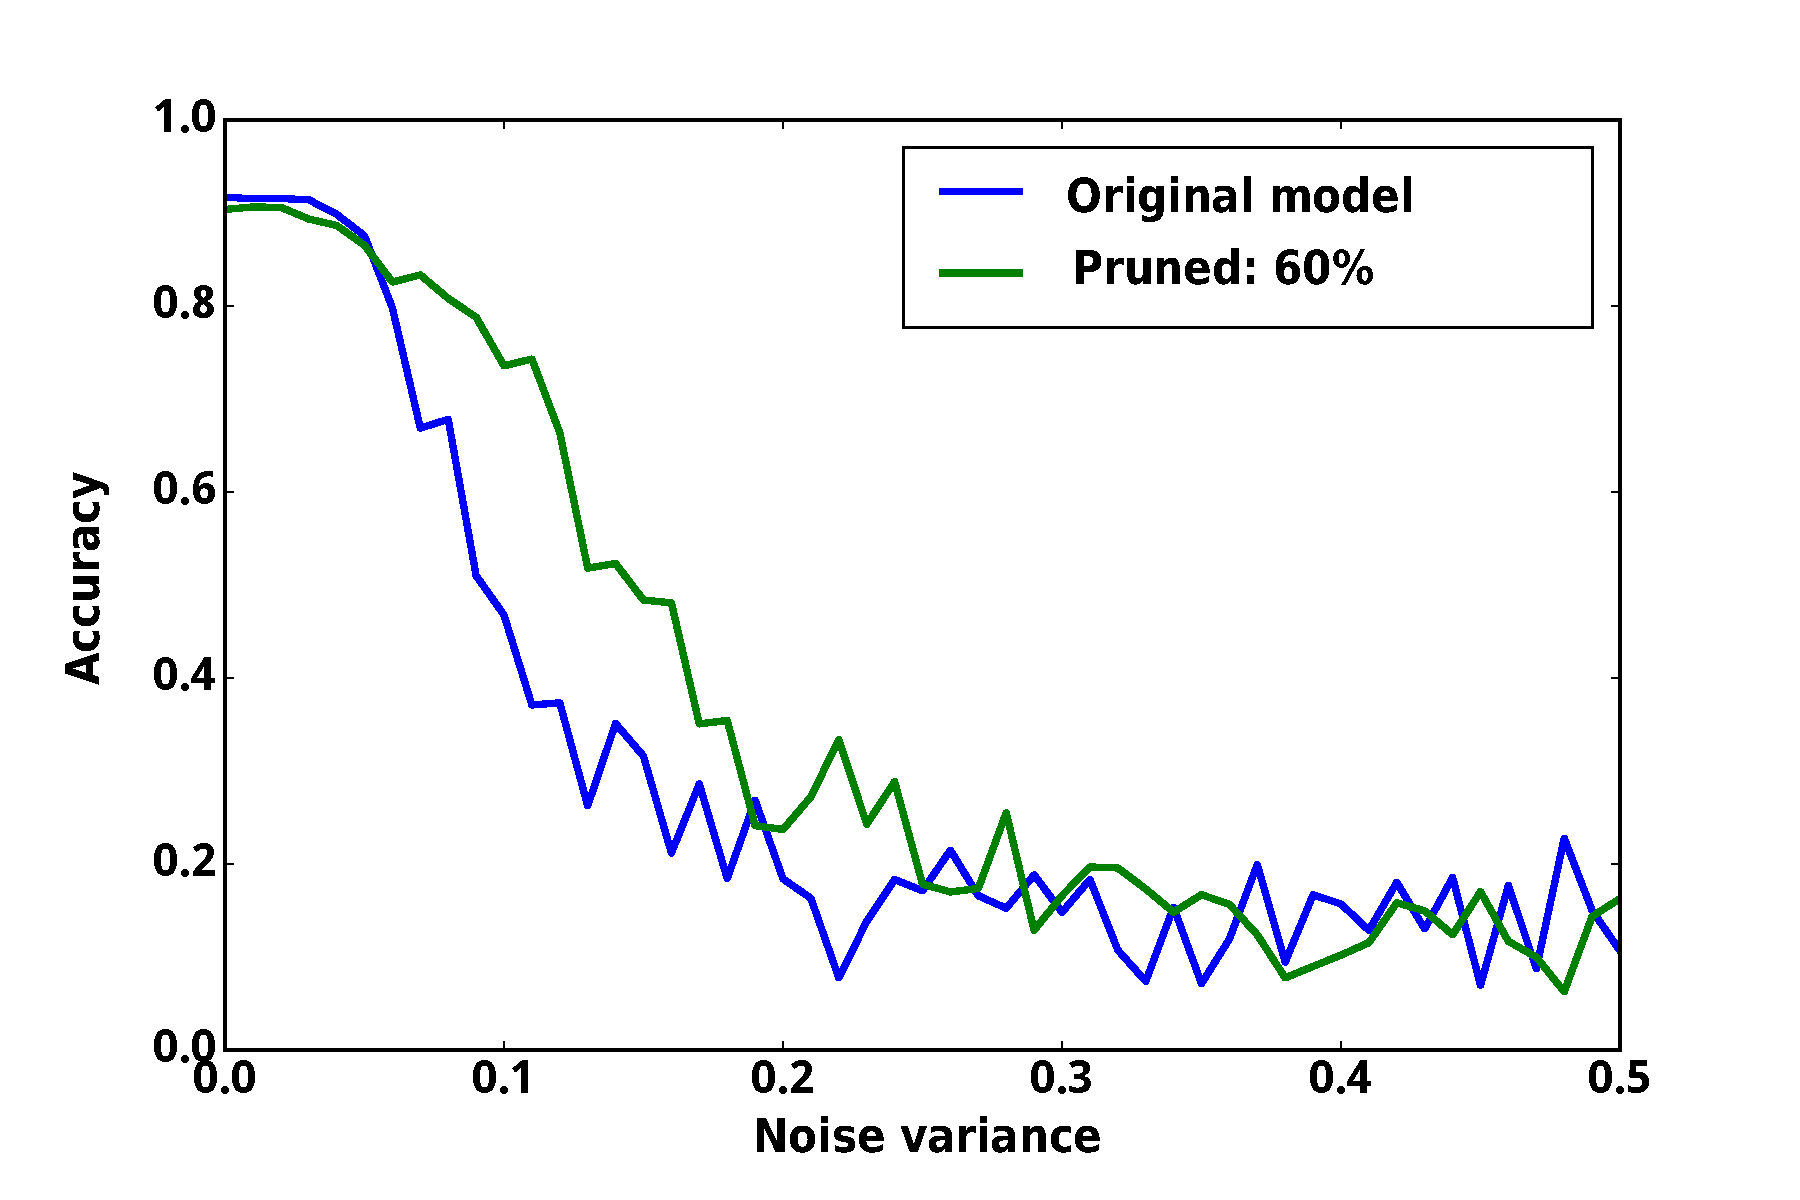
\includegraphics[width=0.55\textwidth]{./slide_plots/noise_en.pdf}}                                                     
\end{figure}                                                                                                   
\textcolor{gray}{Deep learning models have implicitly redundant complexity.}  

                                                                                                                                             
\end{frame}    

\begin{frame}{Deep learning model}
\small
\begin{block}{Definition}
\textit{Model} $\mathbf{f}(\mathbf{w}, \mathbf{x})$ is a differentiable function with respect to parameters $\mathbf{w}$  from the set of object descriptions into the set of labels:
\[
    \mathbf{f}: \mathbb{X} \times \mathbb{W} \to \mathbb{Y},
\] 
where $\mathbb{W}$ is a space of parameters of model $\mathbf{f}$.
\end{block}
~\\
\textbf{Main challenge} of deep learning model selection is in large number of parameters of models. This disallows to use many classical approached for the model and structure selection (AIC, BIC, cross-validation). \\~\\
A model is defined by its parameters $\mathbf{W}$ and structure $\boldsymbol{\Gamma}$.\\
A \textbf{structure} defines a set of functional superpositions in the model. It is selected using statistical complexity criteria.\\

\textbf{Empirical model complexity estimations:}
\begin{enumerate}
\item number of parameters;
\item number of superpositions in the model.
\end{enumerate}
\end{frame}




\begin{frame}{Prior distribution}
\footnotesize   
\begin{columns}
\begin{column}{0.7\textwidth}
   \begin{block}{Definition}
\textit{Prior distribution} for parameters $\mathbf{w}$ and structure $\boldsymbol{\Gamma}$ of model $\mathbf{f}$ is a distribution
$
    \textcolor{red}{p(\mathbf{W}, \boldsymbol{\Gamma}|\mathbf{h},\lam)}: \mathbb{W} \times \amsmathbb{\Gamma} \times \mathbb{H} \to \mathbb{R}^{+}, 
$
where $\mathbb{W}$ is a parameter space, $\amsmathbb{\Gamma}$ is a structure space, $\lam$ is a vector of metaparameters.
\end{block}

\end{column}
\begin{column}{0.25\textwidth}  %%<--- here
    \begin{center}
     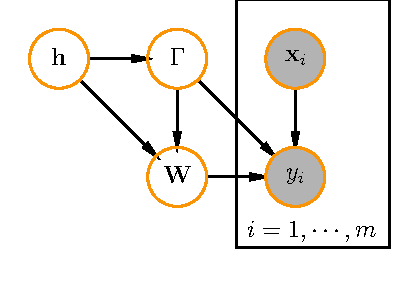
\includegraphics[width=\textwidth]{simple_plate.pdf}
     \end{center}
\end{column}
\end{columns}
\vspace*{-0.5cm}
\begin{block}{Definition}
\textit{Hyperparameters} $\mathbf{h}\in \mathbb{H}$ are the parameters of prior distribution $p(\mathbf{w}, \boldsymbol{\Gamma}|\mathbf{h},\mathbf{f})$ (parameters of the distribution of the parameters and structure  of model $\mathbf{f}$).
 
\end{block}
A model $\mathbf{f}$ is defined by:
\begin{itemize}
\item \textbf{Parameters} $\mathbf{w} \in \mathbb{W}$ that define superpositions  $\mathbf{f}_v$ in the model $\mathbf{f}$.
\item \textbf{Structure} $\boldsymbol{\Gamma}=\{\gamma^{j,k}\}_{(j,k)\in E} \in \amsmathbb{\Gamma}$ that define the contribution of all the superpositions  $\mathbf{f}_v$ into $\mathbf{f}$.
\item \textbf{Hyperparameters} $\mathbf{h} \in \mathbb{H}$ that define the prior distribution.
\item \textbf{Metaparameters} $\boldsymbol{\lambda} \in \amsmathbb{\Lambda}$ that define the optimization function.
\end{itemize}

\end{frame}

\begin{frame}{Model parameters optimization}
\textcolor{blue}{\textbf{Log likelihood:}}
\begin{itemize}
\item $\log p(\mathbf{y}|\mathbf{X}, \mathbf{w}, \mathbf{h}, \mathbf{f}) = \sum_{y, \mathbf{x}} \log p(\mathbf{f}[y]|\mathbf{x}, \mathbf{w}, \mathbf{h}, \mathbf{f})$ for classification problem, \\
where $\mathbf{f}[y]$ is the component   $y$  of the function $y \in \mathcal{N}$.

\item $\log p(\mathbf{y}|\mathbf{X}, \mathbf{w}, \mathbf{h}, \mathbf{f}) = \left(-\frac{1}{2}(\mathbf{f}(\mathbf{X})  -  \mathbf{\mathbf{y}})\mathbf{B}^{-1}(\mathbf{f}(\mathbf{X})  -  \mathbf{\mathbf{y}})^{\mathsf{T}}\right) - \frac{1}{2} |\mathbf{B}| + \text{C},$ for regression problem,\\
where $\mathbf{B}$ is a hyperparameter, $\mathbf{B} \in \mathbf{h}$, $C$ is a constant.
\end{itemize}
\textcolor{red}{\textbf{Prior:}}\\
\begin{itemize}
\item $p(\mathbf{w}|\mathbf{h}) \sim \mathcal{N}(\mathbf{0}, \mathbf{A}^{-1}): \log p(\mathbf{w}|\mathbf{h})  = \left(-\frac{1}{2}(\mathbf{w}\mathbf{A}^{-1}\mathbf{w}{\mathsf{T}})\right) - \frac{1}{2} |\mathbf{A}| + C,$ \\ where $\mathbf{A}$ is a hyperparameter, $\mathbf{B} \in \mathbf{h}$.
\end{itemize}
\end{frame}


\begin{frame}{Structure selection example}
    \begin{table}
        \centering
        \begin{tabular}{ccc}
            hidden layer dim = 1 &   hidden layer dim = 2 &  hidden layer dim = 3 \\
             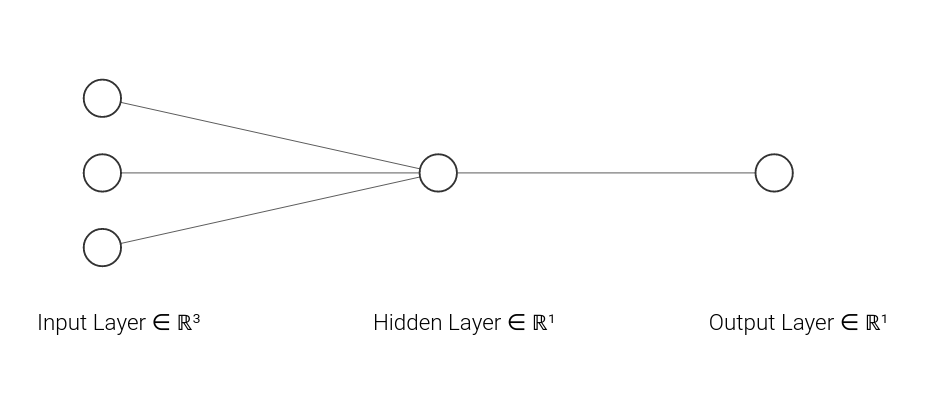
\includegraphics[width=0.33\textwidth]{1node.png} &  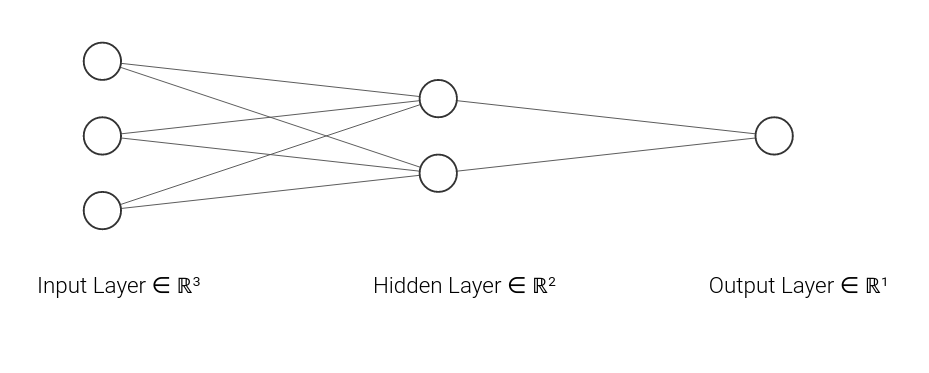
\includegraphics[width=0.3\textwidth]{2node.png} &  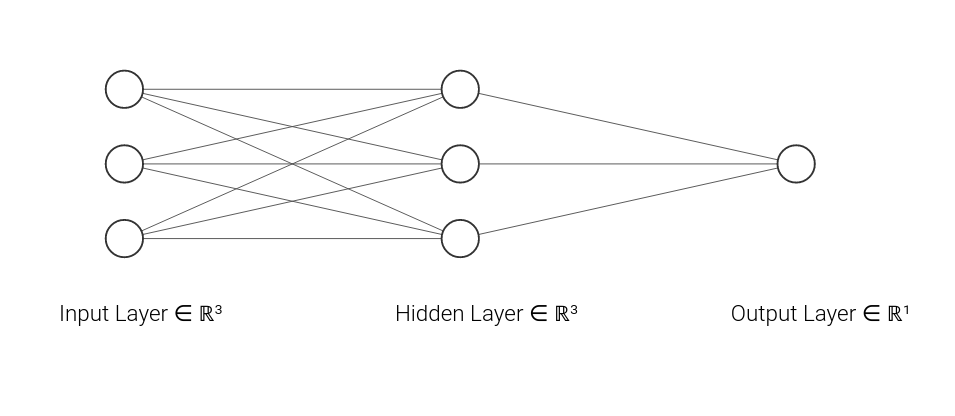
\includegraphics[width=0.33\textwidth]{3node.png} \\
        \end{tabular}


    \end{table}
    \textcolor{gray}{All these models can be represented as $\mathbf{f}(\mathbf{x}, \mathbf{w}) = \boldsymbol{\sigma}\left(\left(\mathbf{w}^2\right)^\mathsf{T}\boldsymbol{\sigma}\left((\mathbf{w}^1)^\mathsf{T}\mathbf{x}\right)\right)$ \\with similar shape of $\mathbf{w}^1: \text{dim}(\mathbf{w}^1) = 3 \times 3.$}
    
\end{frame}

\begin{frame}{Structure selection: one-layer network}
\small
The model $\mathbf{f}$ is defined by the \textbf{structure}  $\boldsymbol{\Gamma} = [\boldsymbol{\gamma}^{0,1}, {\boldsymbol{\gamma}^{1,2}}].$

\[
    \text{Model: }\mathbf{f}(\mathbf{x}) = \textbf{softmax}\left((\mathbf{w}^{1,2}_0)^\mathsf{T}{\mathbf{f}_1}(\mathbf{x})\right), \quad \mathbf{f}(\mathbf{x}): \mathbb{R}^n \to [0,1]^{|\mathbb{Y}|}, \quad \mathbf{x} \in \mathbb{R}^n.
\]
\[
\mathbf{f}_1(\mathbf{x}) = {\gamma}^{0,1}_{0}\mathbf{g}^{0,1}_{0}(\mathbf{x}) + {\gamma}^{0,1}_{1}\mathbf{g}^{0,1}_{1}(\mathbf{x}),
\]
where $\mathbf{w} = [\mathbf{w}^{0,1}_0, \mathbf{w}^{0,1}_1, \mathbf{w}^{1,2}_0]^{\text{T}}$ --- parameter matrices, $\{\mathbf{g}^{0}_{0,1},\mathbf{g}^{1}_{0,1},{\mathbf{g}^{0}_{1,2}\}}$ --- generalized-linear functions, alternatives of layers of the network.

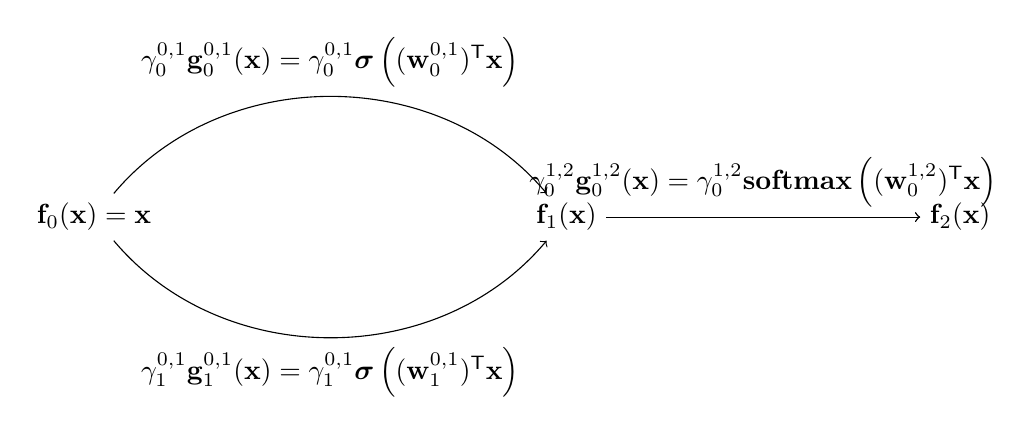
\begin{tikzpicture}[node distance=0.5cm, auto]
  %\tikzstyle{every state}=[fill=red,draw=none,text=white]

  \node (f0)  at (1,6)                  {$\mathbf{f}_0(\mathbf{x}) = \mathbf{x}$};
  %\node (g11) at (6,3)                    {$\mathbf{g}^{1,1}(\mathbf{x})$};% = \text{Conv}(\mathbf{x}, 3, 32, 1)$};
  %\node (g12)  at (6,9)                   {$\mathbf{g}^{1,2}(\mathbf{x})$};% = \text{Conv}(\mathbf{x}, 4, 32, 1)$};
  \node (f1)  at (7,6)                 {$\mathbf{f}_1(\mathbf{x})$};% = \gamma^{1,1}\mathbf{g}^{1,1}(\mathbf{x}) +  \gamma^{1,2}\mathbf{g}^{1,2}(\mathbf{x})$};
  %\node (g21) at (12,6)                   {$\mathbf{g}^{2,1}(\mathbf{x})$};% = \boldsymbol{\sigma}(\mathbf{w}^{2,1}\mathbf{x})$};
  \node (f2)  at (12,6)                   {$\mathbf{f}_2(\mathbf{x})$};% = \gamma^{2,1}\mathbf{g}^{2,1}(\mathbf{x})$};
  \path[->]  (f0) edge [bend left=50] node {$\gamma^{0,1}_0\mathbf{g}^{0,1}_0(\mathbf{x}) = \gamma^{0,1}_0\boldsymbol{\sigma}\left((\mathbf{w}^{0,1}_0)^{\mathsf{T}}\mathbf{x}\right)$}(f1);
  \path[->] (f0)  edge[bend right=50] node[below] {$\gamma^{0,1}_1\mathbf{g}^{0,1}_1(\mathbf{x}) = \gamma^{0,1}_1\boldsymbol{\sigma}\left((\mathbf{w}^{0,1}_1)^{\mathsf{T}}\mathbf{x}\right)$}(f1);
  \path[->] (f1)  edge node {$\gamma^{1,2}_0\mathbf{g}^{1,2}_0(\mathbf{x}) = \gamma^{1,2}_0\textbf{softmax}\left((\mathbf{w}^{1,2}_0)^{\mathsf{T}}\mathbf{x}\right)$}(f2);       
  \draw[->] (f1) to (f2);
 
\end{tikzpicture}

\end{frame}



\begin{frame}{Neural architecture search example}

        \centering
        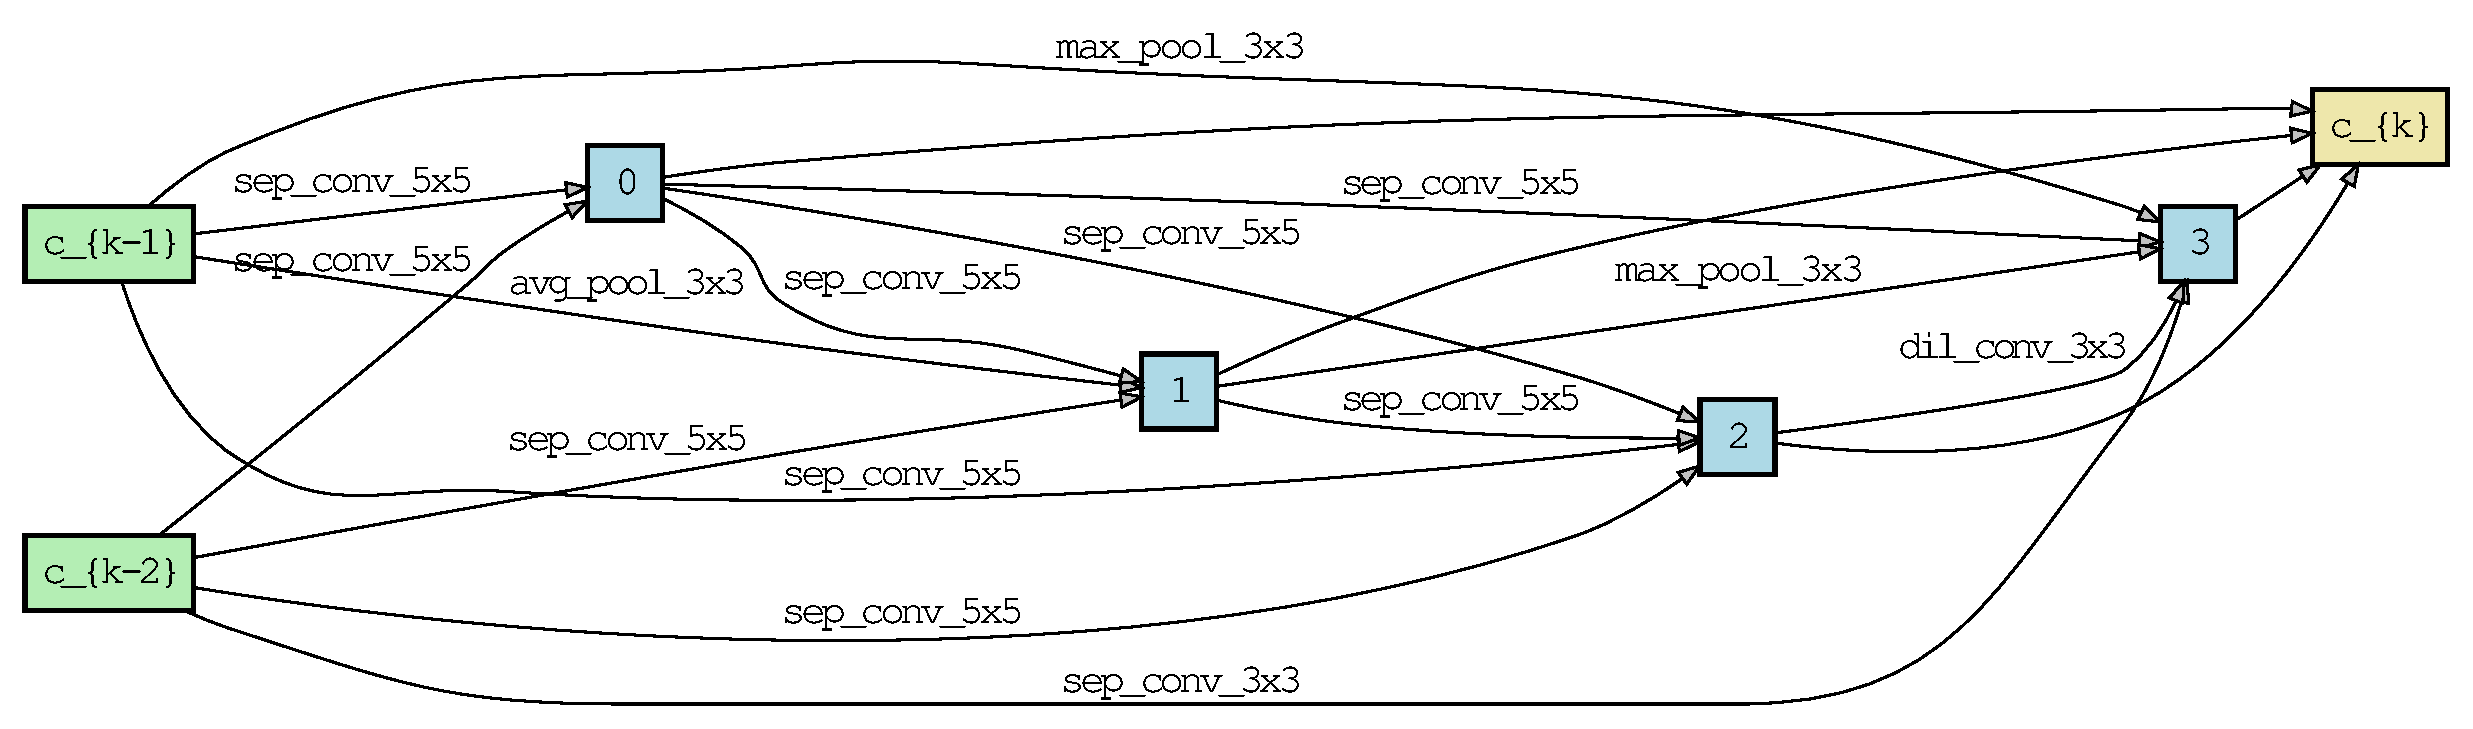
\includegraphics[width=\textwidth]{darts.eps} 
      
    
\end{frame}

\begin{frame}{Structure selection: neural architecture search space}
\small
The model $\mathbf{f}$ is defined by the \textbf{structure}  $\boldsymbol{\Gamma} = [\boldsymbol{\gamma}^{0,1}, {\boldsymbol{\gamma}^{1,2}}].$

\[
    \text{Model: }\mathbf{f}(\mathbf{x}) = \textbf{softmax}\left((\mathbf{w}^{1,2}_0)^\mathsf{T}{\mathbf{f}_1}(\mathbf{x})\right), \quad \mathbf{f}(\mathbf{x}): \mathbb{R}^n \to [0,1]^{|\mathbb{Y}|}, \quad \mathbf{x} \in \mathbb{R}^n.
\]
\[
\mathbf{f}_1(\mathbf{x}) = {\gamma}^{0,1}_{0}\mathbf{g}^{0,1}_{0}(\mathbf{x}) + {\gamma}^{0,1}_{1}\mathbf{g}^{0,1}_{1}(\mathbf{x}),
\]
where $\mathbf{w} = [\mathbf{w}^{0,1}_0, \mathbf{w}^{1,2}_0]^{\text{T}}$ --- parameter matrices, $\mathbf{g}^{0}_{0,1}$ is a convolution,$\mathbf{g}^{1}_{0,1}$ is a pooling operation, $\mathbf{g}^{0}_{1,2}$ is a generalized-linear function.

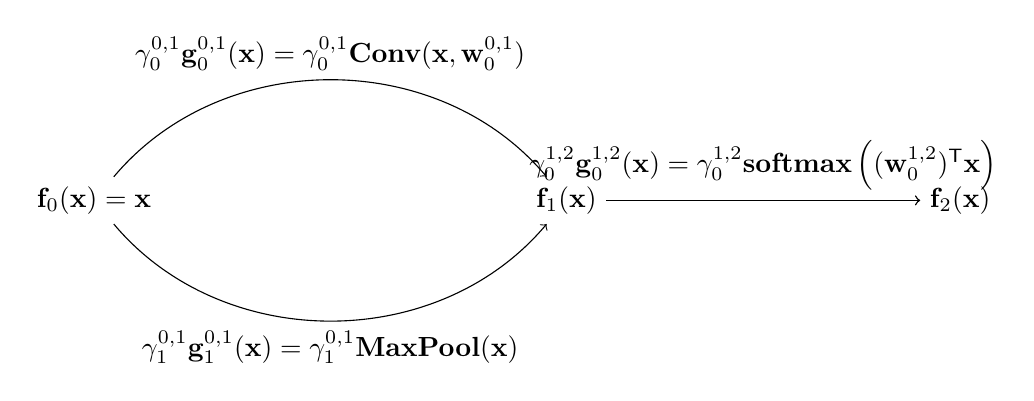
\begin{tikzpicture}[node distance=0.5cm, auto]
  %\tikzstyle{every state}=[fill=red,draw=none,text=white]

  \node (f0)  at (1,6)                  {$\mathbf{f}_0(\mathbf{x}) = \mathbf{x}$};
  %\node (g11) at (6,3)                    {$\mathbf{g}^{1,1}(\mathbf{x})$};% = \text{Conv}(\mathbf{x}, 3, 32, 1)$};
  %\node (g12)  at (6,9)                   {$\mathbf{g}^{1,2}(\mathbf{x})$};% = \text{Conv}(\mathbf{x}, 4, 32, 1)$};
  \node (f1)  at (7,6)                 {$\mathbf{f}_1(\mathbf{x})$};% = \gamma^{1,1}\mathbf{g}^{1,1}(\mathbf{x}) +  \gamma^{1,2}\mathbf{g}^{1,2}(\mathbf{x})$};
  %\node (g21) at (12,6)                   {$\mathbf{g}^{2,1}(\mathbf{x})$};% = \boldsymbol{\sigma}(\mathbf{w}^{2,1}\mathbf{x})$};
  \node (f2)  at (12,6)                   {$\mathbf{f}_2(\mathbf{x})$};% = \gamma^{2,1}\mathbf{g}^{2,1}(\mathbf{x})$};
  \path[->]  (f0) edge [bend left=50] node {$\gamma^{0,1}_0\mathbf{g}^{0,1}_0(\mathbf{x}) = \gamma^{0,1}_0 \textbf{Conv}(\mathbf{x},\mathbf{w}^{0,1}_0)$}(f1);
  \path[->] (f0)  edge[bend right=50] node[below] {$\gamma^{0,1}_1\mathbf{g}^{0,1}_1(\mathbf{x}) = \gamma^{0,1}_1\textbf{MaxPool}(\mathbf{x})$}(f1);
  \path[->] (f1)  edge node {$\gamma^{1,2}_0\mathbf{g}^{1,2}_0(\mathbf{x}) = \gamma^{1,2}_0\textbf{softmax}\left((\mathbf{w}^{1,2}_0)^{\mathsf{T}}\mathbf{x}\right)$}(f2);       
  \draw[->] (f1) to (f2);
 
\end{tikzpicture}

\end{frame}




\begin{frame}{Deep learning model structure as a graph}
\footnotesize
Define:
\begin{enumerate}
 \item acyclic graph $(V,E)$;
\item for each edge $(j,k) \in E$: a vector primitive differentiable functions $\mathbf{g}^{j,k} = [\mathbf{g}^{j,k}_0, \dots, \mathbf{g}^{j,k}_{K^{j,k}}]$  with length of $K^{j,k}$;
\item for each vertex $v \in V$: a differentiable aggregation function  $\textbf{agg}_v$.
\item a function $\mathbf{f} = \mathbf{f}_{|V|-1}:$
\begin{equation}
\label{eq:modelfam}
    \mathbf{f}_{v}(\mathbf{w}, \mathbf{x}) = \textbf{agg}_{v}\left(\{ \langle \boldsymbol{\gamma}^{j,k}, \mathbf{g}^{j,k} \rangle \circ  \mathbf{f}_j(\mathbf{x})| j \in \text{Adj}(v_k)\}\right), v \in \{1,\dots,|V|-1\}, \quad \mathbf{f}_0(\mathbf{x}) = \mathbf{x}
\end{equation}
that is a function from  $\mathbb{X}$ into a set of labels $\mathbb{Y}$ for any value of  $\boldsymbol{\gamma}^{j,k} \in [0,1]^{K^{j,k}}$.
\end{enumerate}

\begin{block}{Definition}
A \textit{parametric set of models} $\mathfrak{F}$ is a graph $(V, E)$  with a set of primitive functions $\{\mathbf{g}^{j,k}, (j,k) \in E\}$ and aggregation functions  $\{ \textbf{agg}_v, {v \in V}\}$.
\end{block}
\begin{block}{Statement}
A function $\mathbf{f} \in \mathfrak{F}$ is a model for each  $\boldsymbol{\gamma}^{j,k} \in [0,1]^{K^{j,k}}$.
\end{block}
\end{frame}




\begin{frame}{Structure restrictions}
An example of restrictions for structure parameter $\boldsymbol{\gamma}$, $|\boldsymbol{\gamma}| = 3$.
\begin{figure}
 \begin{minipage}[t]{.45\textwidth}
        \centering
%1 limit
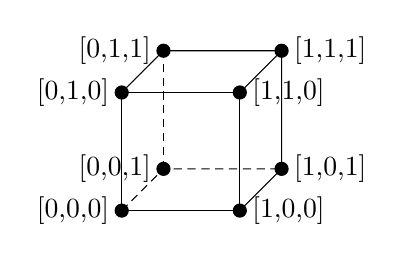
\begin{tikzpicture}[%
x={(1.5cm,0cm)},
y={(0cm,1.5cm)},
z={({0.5*cos(45)},{0.5*sin(45)})},
]

\coordinate (A) at (0,0,0); 
\coordinate (B) at (1,0,0) ;
\coordinate (C) at (1,1,0); 
\coordinate (D) at (0,1,0); 
\coordinate (E) at (0,0,1); 
\coordinate (F) at (1,0,1); 
\coordinate (G) at (1,1,1); 
\coordinate (H) at (0,1,1   );

%Ecken
\node[circle,scale=0.5,fill=black,draw=black](Ap) at (0,0,0){};
\node[circle,scale=0.5,fill=black,draw=black](Bp) at (1,0,0){};
\node[circle,scale=0.5,fill=black,draw=black](Cp) at (1,1,0){};
\node[circle,scale=0.5,fill=black,draw=black](Dp) at (0,1,0){};
\node[circle,scale=0.5,fill=black,draw=black](Ep) at (0,0,1){};
\node[circle,scale=0.5,fill=black,draw=black](Fp) at (1,0,1){};
\node[circle,scale=0.5,fill=black,draw=black](Gp) at (1,1,1){};
\node[circle,scale=0.5,fill=black,draw=black](Hp) at (0,1,1){};
\node[left= 1pt of A]{[0,0,0]};
\node[right= 1pt of B]{[1,0,0]};
\node[right= 1pt of C]{[1,1,0]};
\node[left= 1pt of D]{[0,1,0]};
\node[left= 1pt of E]{[0,0,1]};
\node[right= 1pt of F]{[1,0,1]};
\node[right= 1pt of G]{[1,1,1]};
\node[left= 1pt of H]{[0,1,1]};

%Kanten
\draw[] (A)
-- (B)  node[midway, below]{}
-- (C)      node[midway, right]{}
-- (D)  node[midway, above]{}
-- (A)  node[midway, left]{};
\draw[] (B) -- (F) -- (G) -- (C);
\draw[] (G) -- (H) -- (D);
\draw[densely dashed] (A) -- (E) -- (F);
\draw[densely dashed] (E) -- (H);

\end{tikzpicture}
\caption*{Cube vertices}
\end{minipage}
\hfill
 \begin{minipage}[t]{.45\textwidth}
        \centering

%2 limit
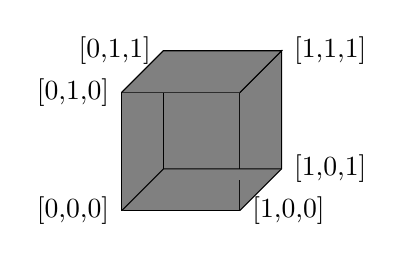
\begin{tikzpicture}[%
x={(1.5cm,0cm)},
y={(0cm,1.5cm)},
z={({0.5*cos(45)},{0.5*sin(45)})},
]

\coordinate (A) at (0,0,0); 
\coordinate (B) at (1,0,0) ;
\coordinate (C) at (1,1,0); 
\coordinate (D) at (0,1,0); 
\coordinate (E) at (0,0,1); 
\coordinate (F) at (1,0,1); 
\coordinate (G) at (1,1,1); 
\coordinate (H) at (0,1,1   );

%Ecken
\node[left= 1pt of A]{[0,0,0]};
\node[right= 1pt of B]{[1,0,0]};
\node[right= 1pt of C]{};
\node[left= 1pt of D]{[0,1,0]};
\node[left= 1pt of E]{};
\node[right= 1pt of F]{[1,0,1]};
\node[right= 1pt of G]{[1,1,1]};
\node[left= 1pt of H]{[0,1,1]};

%Kanten
\draw[fill=gray] (A)
-- (B)  node[midway, below]{}
-- (C)      node[midway, right]{}
-- (D)  node[midway, above]{}
-- (A)  node[midway, left]{};
\draw[fill=gray] (B) -- (F) -- (G) -- (C);
\draw[fill=gray] (G) -- (H) -- (D);
\draw[fill=gray] (A) -- (E) -- (F);
\draw[fill=gray] (E) -- (H);
\draw[fill=gray] (D) -- (H) -- (G) -- (C);
\end{tikzpicture}
\caption*{Cube interior}
\end{minipage}
\hfill
 \begin{minipage}[t]{.45\textwidth}
        \centering
%3 limit
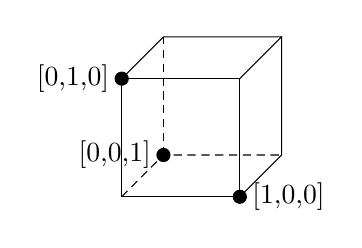
\begin{tikzpicture}[%
x={(1.5cm,0cm)},
y={(0cm,1.5cm)},
z={({0.5*cos(45)},{0.5*sin(45)})},
]

\coordinate (A) at (0,0,0); 
\coordinate (B) at (1,0,0) ;
\coordinate (C) at (1,1,0); 
\coordinate (D) at (0,1,0); 
\coordinate (E) at (0,0,1); 
\coordinate (F) at (1,0,1); 
\coordinate (G) at (1,1,1); 
\coordinate (H) at (0,1,1   );

%Ecken
\node[circle,scale=0.5,fill=black,draw=black](Bp) at (1,0,0){};
\node[circle,scale=0.5,fill=black,draw=black](Dp) at (0,1,0){};
\node[circle,scale=0.5,fill=black,draw=black](Ep) at (0,0,1){};
\node[left= 1pt of A]{};
\node[right= 1pt of B]{[1,0,0]};
\node[right= 1pt of C]{};
\node[left= 1pt of D]{[0,1,0]};
\node[left= 1pt of E]{[0,0,1]};
\node[right= 1pt of F]{};
\node[right= 1pt of G]{};
\node[left= 1pt of H]{};

%Kanten
\draw[] (A)
-- (B)  node[midway, below]{}
-- (C)      node[midway, right]{}
-- (D)  node[midway, above]{}
-- (A)  node[midway, left]{};
\draw[] (B) -- (F) -- (G) -- (C);
\draw[] (G) -- (H) -- (D);
\draw[densely dashed] (A) -- (E) -- (F);
\draw[densely dashed] (E) -- (H);

\end{tikzpicture}
\caption*{Simplex vertices}
\end{minipage}
\hfill
 \begin{minipage}[t]{.45\textwidth}
        \centering
%4 limit
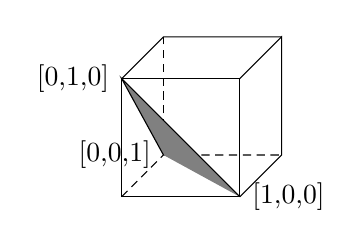
\begin{tikzpicture}[%
x={(1.5cm,0cm)},
y={(0cm,1.5cm)},
z={({0.5*cos(45)},{0.5*sin(45)})},
]

\coordinate (A) at (0,0,0); 
\coordinate (B) at (1,0,0) ;
\coordinate (C) at (1,1,0); 
\coordinate (D) at (0,1,0); 
\coordinate (E) at (0,0,1); 
\coordinate (F) at (1,0,1); 
\coordinate (G) at (1,1,1); 
\coordinate (H) at (0,1,1   );

%Ecken
\node[left= 1pt of A]{};
\node[right= 1pt of B]{[1,0,0]};
\node[right= 1pt of C]{};
\node[left= 1pt of D]{[0,1,0]};
\node[left= 1pt of E]{[0,0,1]};
\node[right= 1pt of F]{};
\node[right= 1pt of G]{};
\node[left= 1pt of H]{};

%Kanten
\draw[] (A)
-- (B)  node[midway, below]{}
-- (C)      node[midway, right]{}
-- (D)  node[midway, above]{}
-- (A)  node[midway, left]{};
\draw[] (B) -- (F) -- (G) -- (C);
\draw[] (G) -- (H) -- (D);
\draw[densely dashed] (A) -- (E) -- (F);
\draw[densely dashed] (E) -- (H);
\draw[fill=gray] (B) -- (D) -- (E);


\end{tikzpicture}
\caption*{Simplex interior}
\end{minipage}

\end{figure}

\end{frame}









\begin{frame}{Prior distribution for the model structure}
Every point in a simplex defines a model.

\textbf{Gumbel-Softmax distribution: }$\textcolor{red}{\boldsymbol{\Gamma}\sim \text{GS}(\mathbf{s}, \lambda_\text{temp})}$\\
\begin{figure}
 \begin{minipage}[t]{.2\textwidth}
        \centering
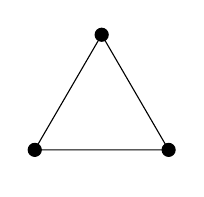
\begin{tikzpicture}[%
x={(1.7cm,0cm)},
y={(0cm,1.7cm)},
]

\coordinate (A) at (0,0); 
\coordinate (B) at (1,0) ;
\coordinate (C) at (0.5,0.86); 

%Ecken
\node[circle,scale=0.5,fill=black,draw=black](Ap) at (0,0){};
\node[circle,scale=0.5,fill=black,draw=black](Bp) at (1,0){};
\node[circle,scale=0.5,fill=black,draw=black](Cp) at (0.5,0.86){};

%Kanten
\draw[] (A)
-- (B)  node[midway, below]{}
-- (C)      node[midway, right]{}
-- (A)  node[midway, left]{};

\end{tikzpicture}
\caption*{$\lambda_\text{temp}\to0$}
\end{minipage}
\hfill
 \begin{minipage}[t]{.2\textwidth}
   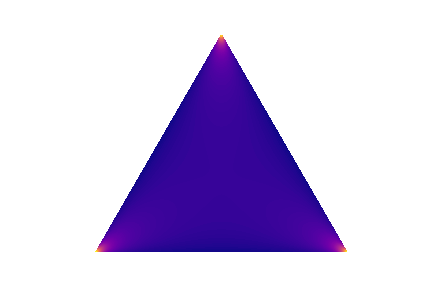
\includegraphics[width=\textwidth]{gs0995.png}
\caption*{$\lambda_\text{temp}=0.995$}
\end{minipage}
\hfill
 \begin{minipage}[t]{.2\textwidth}
   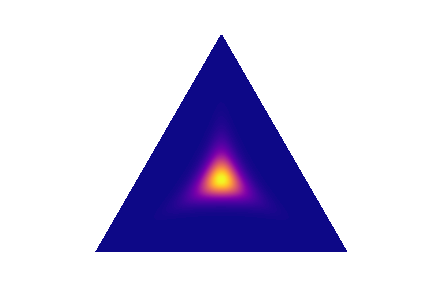
\includegraphics[width=\textwidth]{gs5.png}
\caption*{$\lambda_\text{temp}=5.0$}
\end{minipage}

\end{figure}

\textbf{Dirichlet distribution: }$\textcolor{red}{\boldsymbol{\Gamma}\sim \text{Dir}(\mathbf{s}, \lambda_\text{temp})}$\\
\begin{figure}
 \begin{minipage}[t]{.2\textwidth}
        \centering
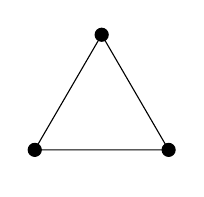
\begin{tikzpicture}[%
x={(1.7cm,0cm)},
y={(0cm,1.7cm)},
]

\coordinate (A) at (0,0); 
\coordinate (B) at (1,0) ;
\coordinate (C) at (0.5,0.86); 

%Ecken
\node[circle,scale=0.5,fill=black,draw=black](Ap) at (0,0){};
\node[circle,scale=0.5,fill=black,draw=black](Bp) at (1,0){};
\node[circle,scale=0.5,fill=black,draw=black](Cp) at (0.5,0.86){};

%Kanten
\draw[] (A)
-- (B)  node[midway, below]{}
-- (C)      node[midway, right]{}
-- (A)  node[midway, left]{};

\end{tikzpicture}
\caption*{$\lambda_\text{temp}\to0$}
\end{minipage}
\hfill
 \begin{minipage}[t]{.2\textwidth}
   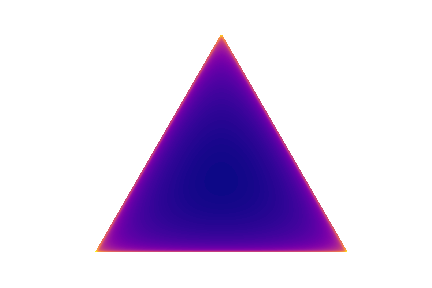
\includegraphics[width=\textwidth]{dir0995.png}
\caption*{$\lambda_\text{temp}=0.995$}
\end{minipage}
\hfill
 \begin{minipage}[t]{.2\textwidth}
   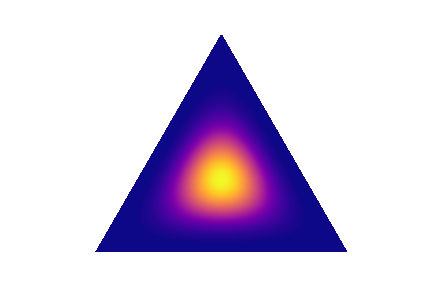
\includegraphics[width=\textwidth]{dir5.png}
\caption*{$\lambda_\text{temp}=5.0$}
\end{minipage}

\end{figure}

\end{frame}







\begin{frame}{Bayesian model selection}


\begin{columns}
\begin{column}{0.6\textwidth}
\begin{itemize}
\item \textbf{parameters} \\ $\textcolor{red}{\mathbf{w}_r^{j,k} \sim \mathcal{N}(0, (\mathbf{A}_r^{j,k})^{-1})},$
$\mathbf{A}_r^{j,k}$ is a diagonal matrix for the parameters of the primitive function $\mathbf{g}_r^{j,k}$,
\item \textbf{structure} \\$\boldsymbol{\Gamma} = \{\boldsymbol{\gamma}^{j,k}, (j,k) \in E\},$ \\$\textcolor{red}{\boldsymbol{\gamma}^{j,k} \sim \text{GS}(\mathbf{s}^{j,k}, \lambda_\text{temp})},$ 
\item \textbf{hyperparameters} $\mathbf{h} = [\text{diag}(\mathbf{A}), \mathbf{s} ],$
\item \textbf{metaparameters} $\lambda_\text{temp}$.
\end{itemize}

\end{column}


\begin{column}{0.4\textwidth}
\begin{figure}
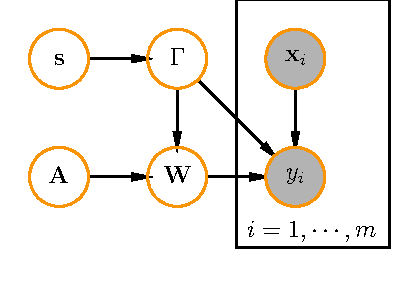
\includegraphics[width=\textwidth]{simple_plate_concrete.pdf}
\end{figure}
\end{column}

\end{columns}

%

\end{frame}



\begin{frame}{Evidence as a statistical complexity}  
\footnotesize
\textbf{Minimum description length} for the model $\mathbf{f}$:
\[
	\text{MDL}(\mathbf{y},\mathbf{f}) = \textcolor{OliveGreen}{-\text{log}~p(\mathbf{h}|\mathbf{f})} - \textcolor{red}{\text{log}~p(\hat{\mathbf{w}} | \mathbf{h},\mathbf{f})}-  \textcolor{blue}{\text{log}~\bigl(p(\mathbf{y}|\mathbf{X}, \hat{\mathbf{w}},\mathbf{f})\delta\mathfrak{D}\bigr)},
\]
where $\delta\mathfrak{D}$ is an information transmission precision.\\
\textbf{Bayesian approach:}\\
Obtain values of parameters   $\mathbf{w}$ with respect to \textbf{posterior distribution of parameters}:                                      
\[
     L = \text{log} p(\mathbf{w}|\mathbf{X}, \mathbf{y}, \mathbf{h}, \lam) \propto  \textcolor{red}{\text{log} p(\mathbf{y}|\mathbf{X},\mathbf{w}, \mathbf{h},\lam)} +  \textcolor{blue}{\text{log} p(\mathbf{w} |\mathbf{h},\lam)}.
\]

Hyperparameters are optimized using  \textbf{posterior distribution of hyperparameters}:                                      
\[                                                                                                                                              
        Q = \text{log}p(\mathbf{f}|\mathbf{X}, \mathbf{y}) \propto \textcolor{OliveGreen}{\text{log}p(\mathbf{h}|\mathbf{f})} +  \text{log}\int\limits_{\mathbf{w}} \textcolor{red}{p(\mathbf{y}|\mathbf{X},\mathbf{w},\lam)} \textcolor{blue}{p(\mathbf{w}| \mathbf{h},\lam)} d\mathbf{w}.                     
\]       

\end{frame}

\begin{frame}{Evidence: example}
\begin{figure}
\vspace{-0.5cm}
  \centering    
 \subfloat[]{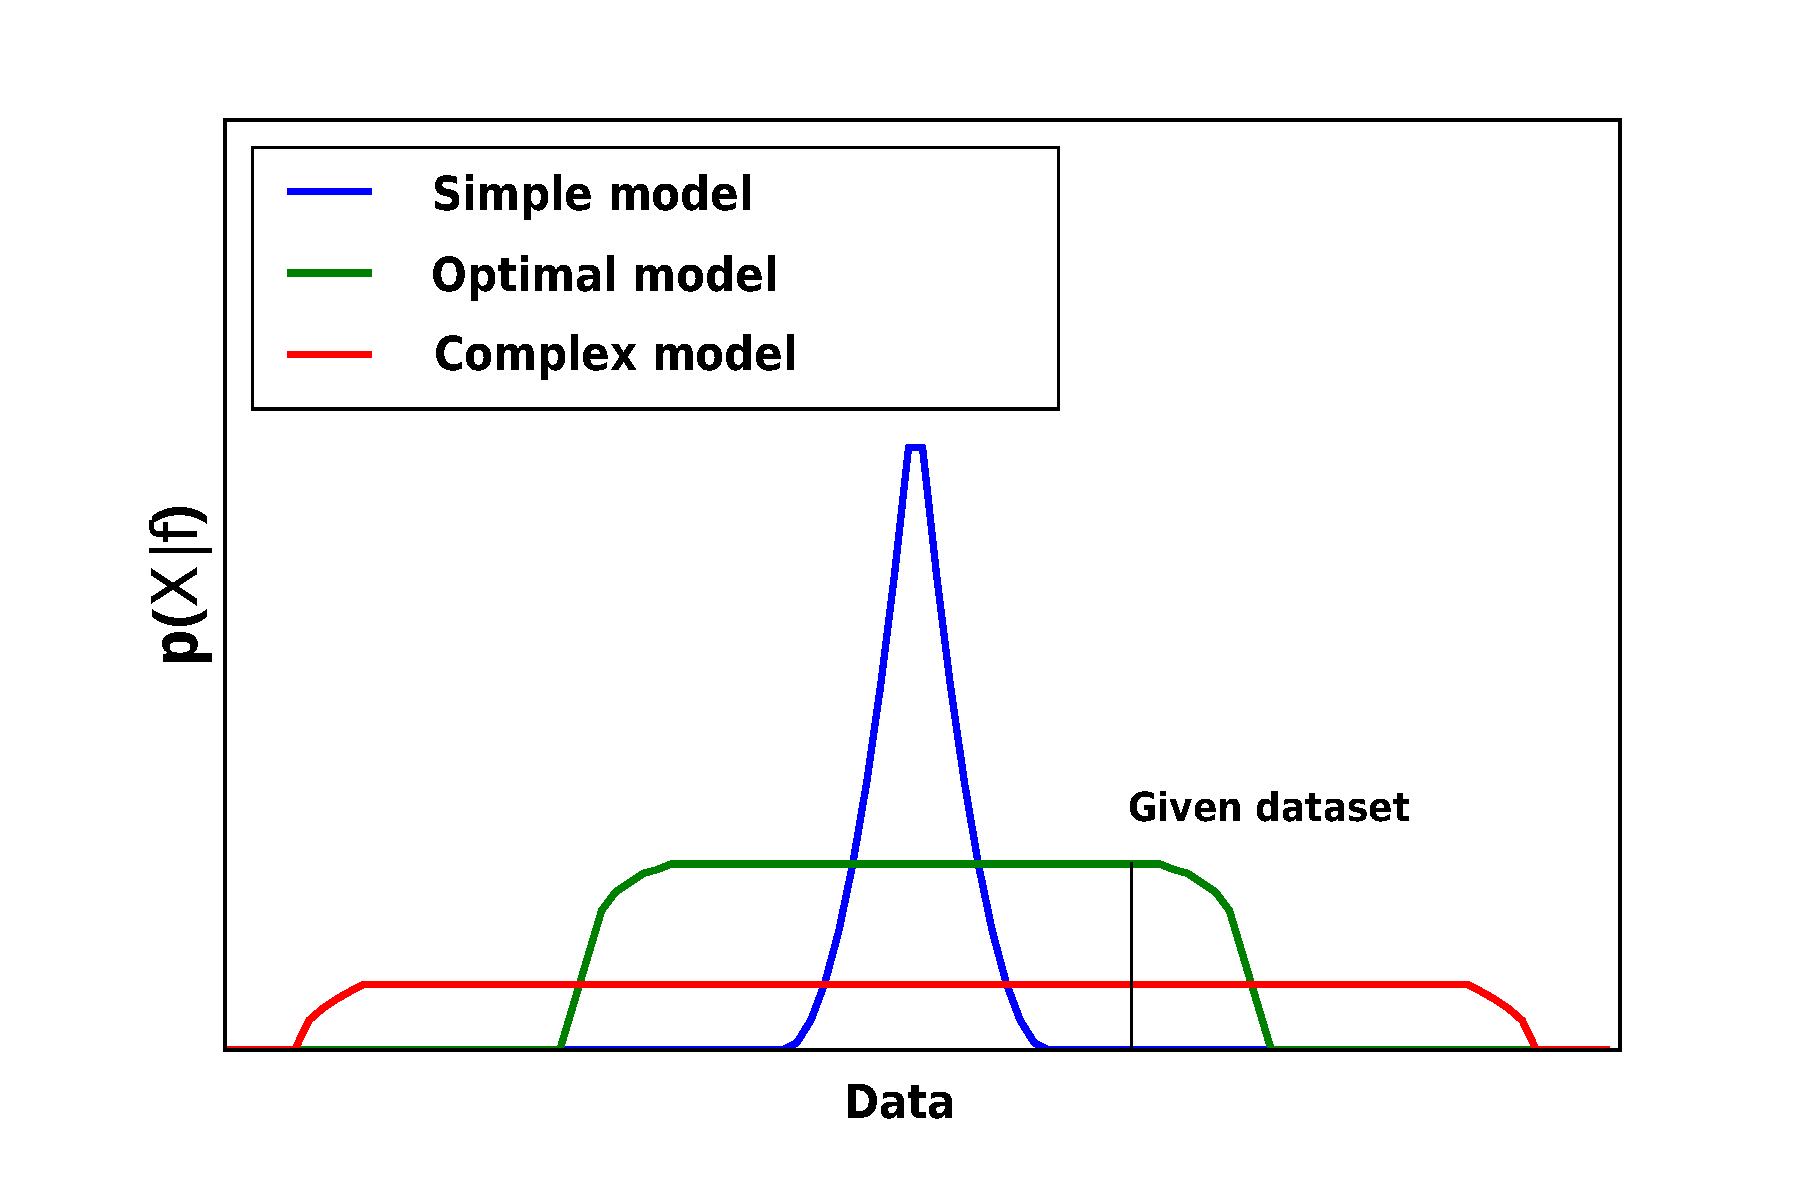
\includegraphics[width=0.5\textwidth]{slide_plots/evidence_en.pdf}} 
 \subfloat[]{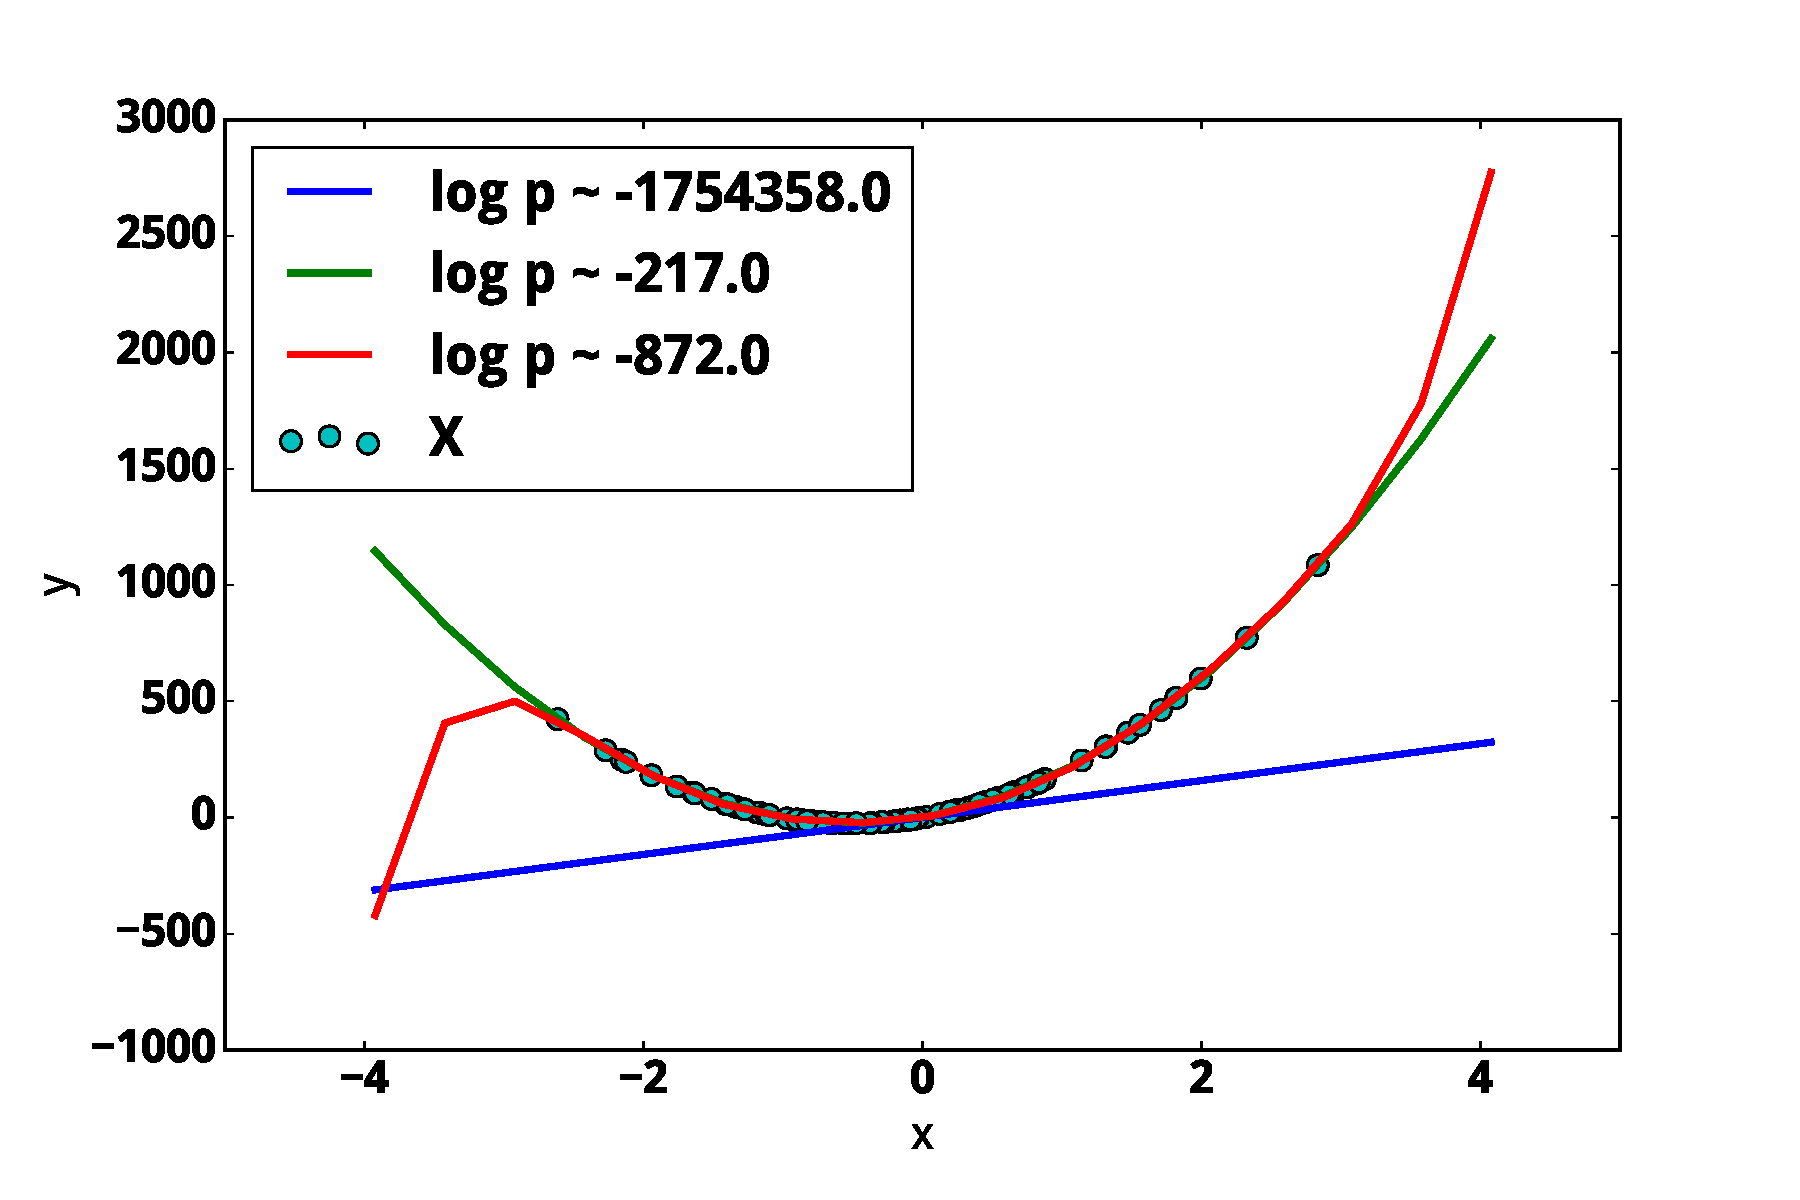
\includegraphics[width=0.5\textwidth]{slide_plots/example.pdf}}

\end{figure}
\end{frame}


\begin{frame}{Evidence lower bound} 
\footnotesize
The evidence is analytically intractable.\\
\textbf{Model evidence:}
\[
p(\mathbf{y}|\mathbf{X}, \h, \lam) =
 \iint\limits_{\mathbf{w}, \boldsymbol{\Gamma}}  \textcolor{red}{p(\mathbf{y}|\mathbf{X},\mathbf{w},  \boldsymbol{\Gamma})} \textcolor{blue}{p(\mathbf{w}, \boldsymbol{\Gamma}|\mathbf{h}, \lam)}d\mathbf{w}d{\boldsymbol{\Gamma}}.                         
\]

\begin{columns}
\begin{column}{0.55\textwidth}
  
\begin{block}{Definition}
\textit{Variational parameters} of the model $\boldsymbol{\theta} \in \Tetab$ are the parameters of the distribution $q$ that approximates posterior distribution $p(\mathbf{w}, \boldsymbol{\Gamma}|\mathbf{X}, \mathbf{y}, \mathbf{h}, \lam)$:
\[
    q \approx  \frac{\textcolor{blue}{p(\mathbf{y}|\mathbf{X},\mathbf{w},\boldsymbol{\Gamma})}\textcolor{red}{p(\mathbf{w}, \boldsymbol{\Gamma}|\mathbf{h}, \lam)}}{\iint\limits_{\mathbf{w}', \boldsymbol{\Gamma'}}\textcolor{blue}{p(\mathbf{y}|\mathbf{X},\mathbf{w}',\boldsymbol{\Gamma}')}\textcolor{red}{p(\mathbf{w}', \boldsymbol{\Gamma}'|\mathbf{h}, \lam)}d\mathbf{w}'d\boldsymbol{\Gamma}'}.
\]
\end{block} 

\end{column}
\begin{column}{0.45\textwidth}  %%<--- here
    \begin{center}
     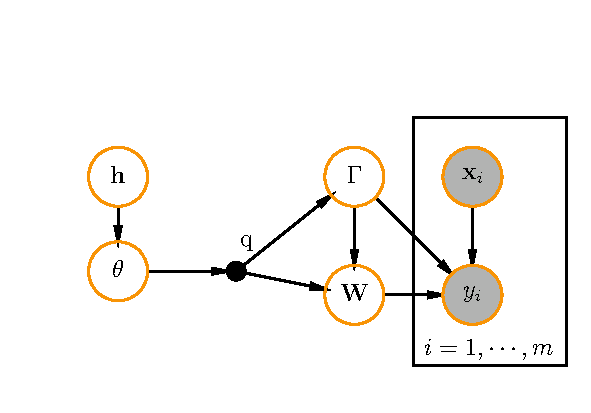
\includegraphics[width=\textwidth]{plate.pdf}
     \end{center}
\end{column}
\end{columns}



%Пусть $q(\mathbf{W}, \boldsymbol{\Gamma}) = q_{\mathbf{W}}(\mathbf{W})q_{\boldsymbol{\Gamma}}(\boldsymbol{\Gamma})$ --- непрерывное распределение, аппроксимирующее 
%апостериорное распределение $p(\mathbf{W}, \boldsymbol{\Gamma}|\mathbf{y}, \mathbf{X})$.
~\\Lower bound of $\text{log}{{p}}(\mathbf{y}|\mathbf{X}, \h, \lam)$:
$$                                                                                                                                              
        \text{log}~p(\mathbf{y}|\mathbf{X}, \h, \lam) \geq 
\textcolor{blue}{\mathsf{E}_q \text{log}~{p(\mathbf{y} | \mathbf{X}, \mathbf{w}, \boldsymbol{\Gamma})}} - \textcolor{red}{\text{D}_{KL}\bigl(q(\mathbf{w}, \boldsymbol{\Gamma})||p(\mathbf{w}, \boldsymbol{\Gamma}| \mathbf{h}, \lam)\bigr)}.
$$ 



The lower bound equals to evidence when $$D_\text{KL}\bigl(q(\mathbf{w}, \boldsymbol{\Gamma})|p\left(\mathbf{w}, \boldsymbol{\Gamma}|\mathbf{y}, \mathbf{X}, \h, \lam\right)\bigr)=0.$$

\end{frame}      




\begin{frame}

\frametitle{Gradient descent as an evidence lower bound}
\footnotesize
Empirical distribtuion of the optimized model parameters is a variational distribution.\\


\begin{multicols}{2}
Gradient descent does not optimize evidence lower bound.
\vspace{-1.cm}
\begin{figure}

\subfloat{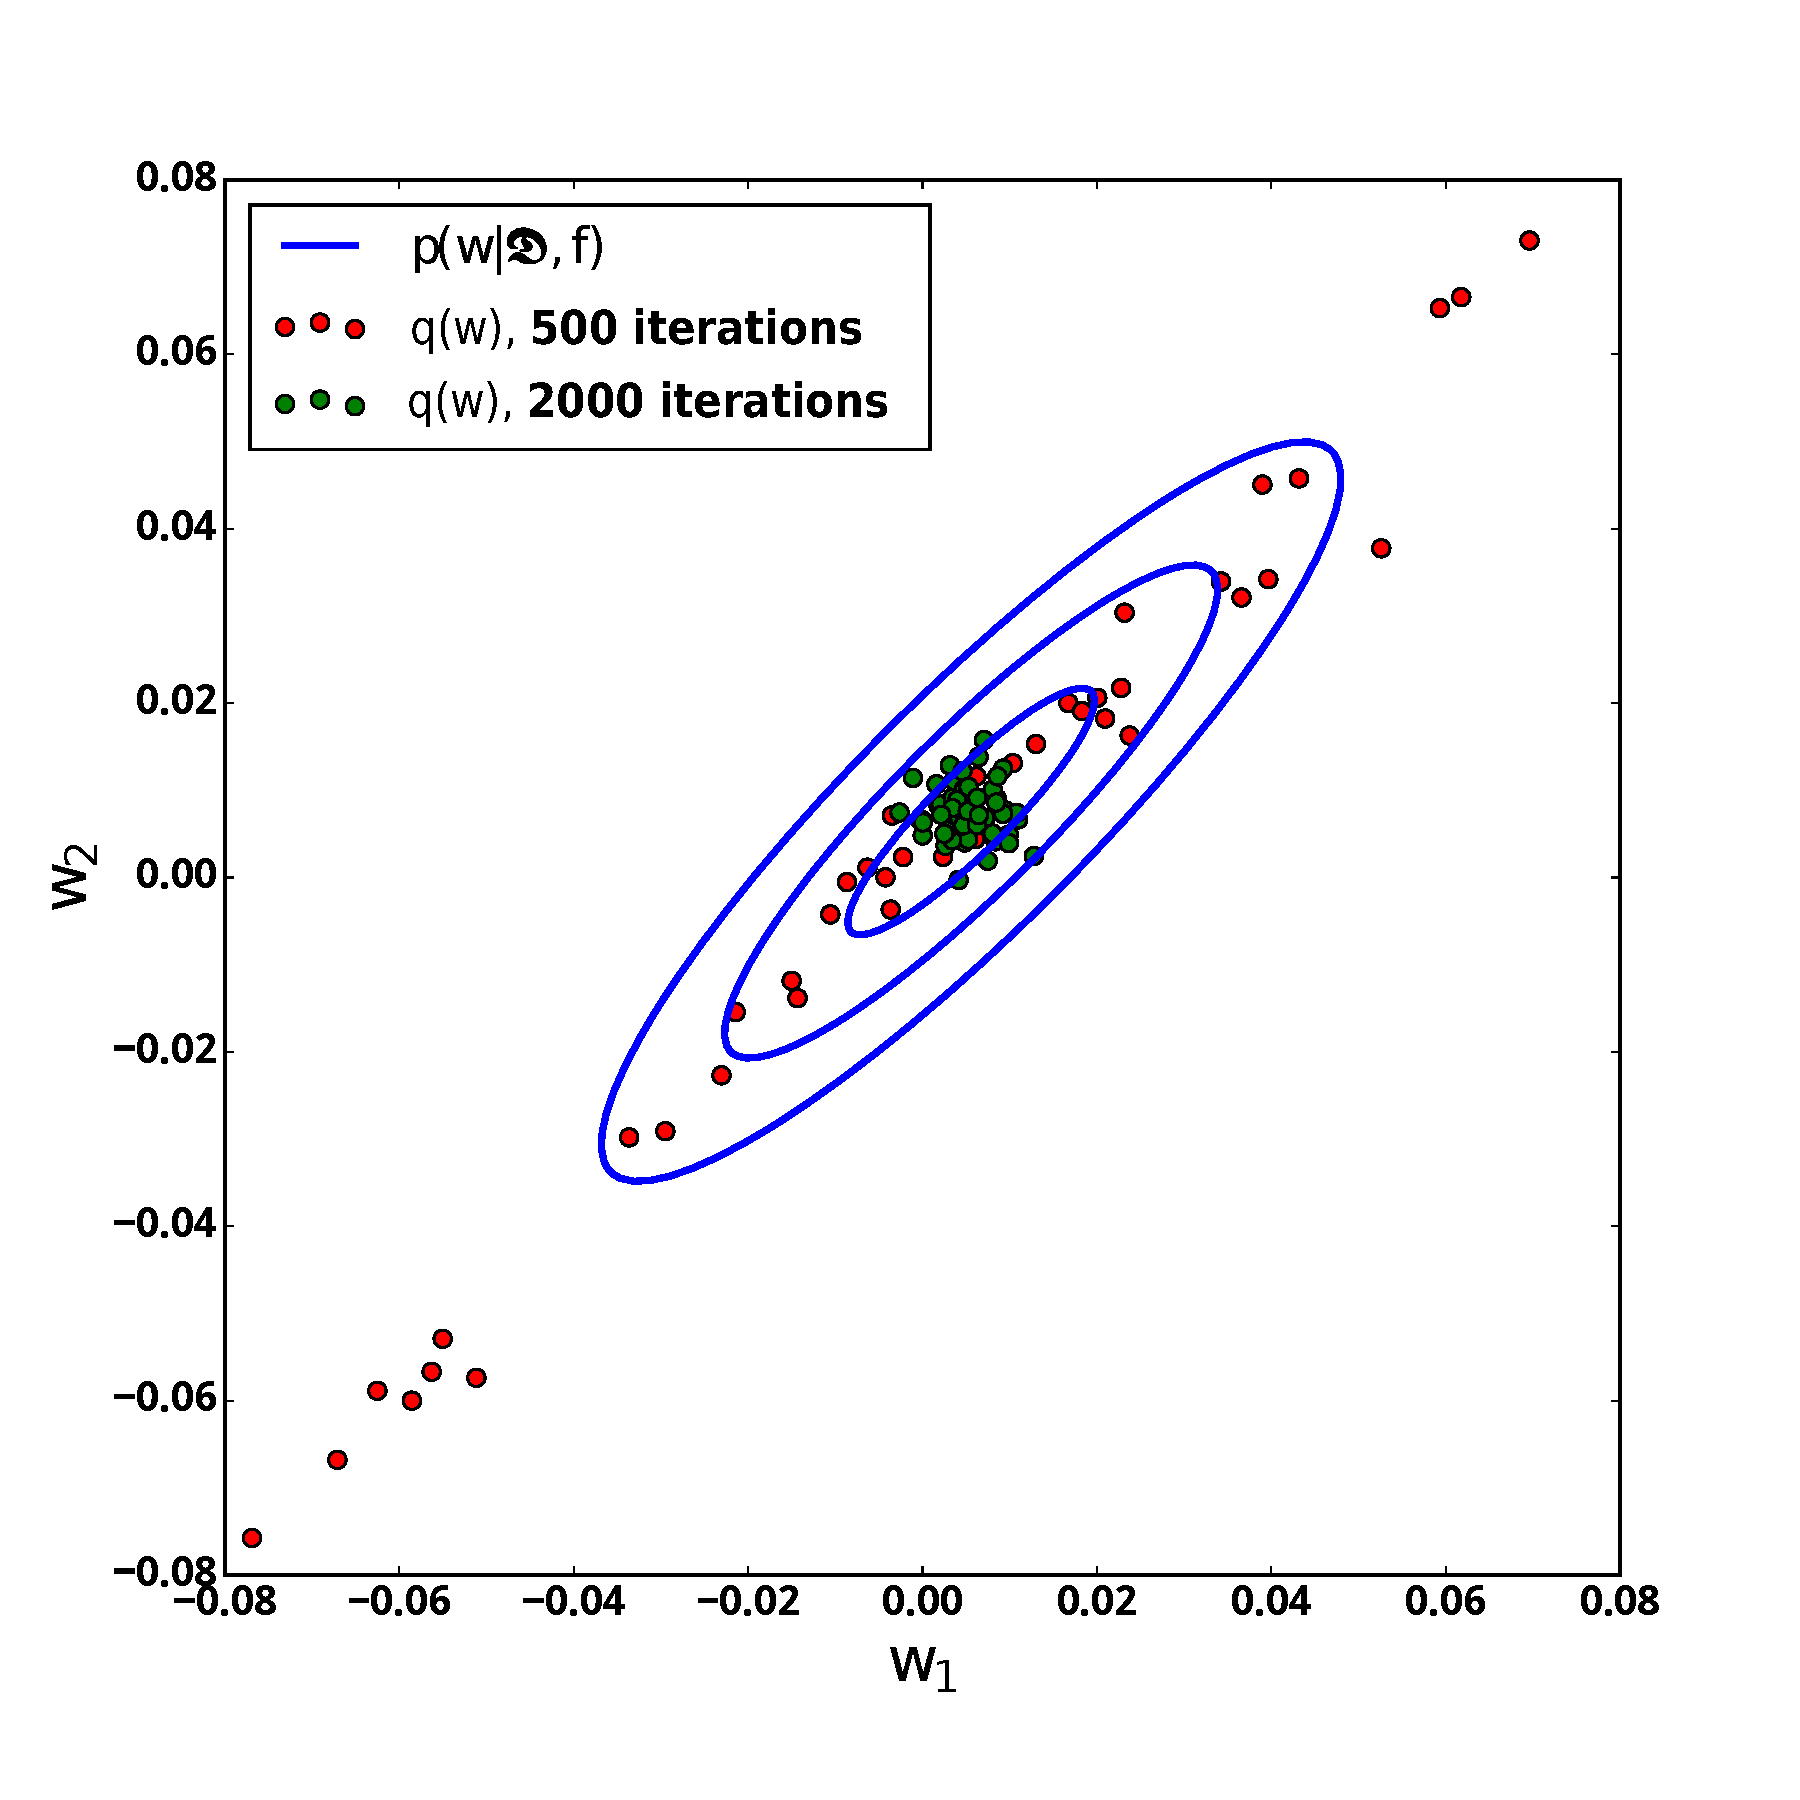
\includegraphics[width=0.4\textwidth]{./slide_plots/sgd_estimate_en.pdf}}
\end{figure}

\columnbreak

Evidence lower bound decrease is a signal of overfitting.
\vspace{0.2cm}
\begin{figure}
{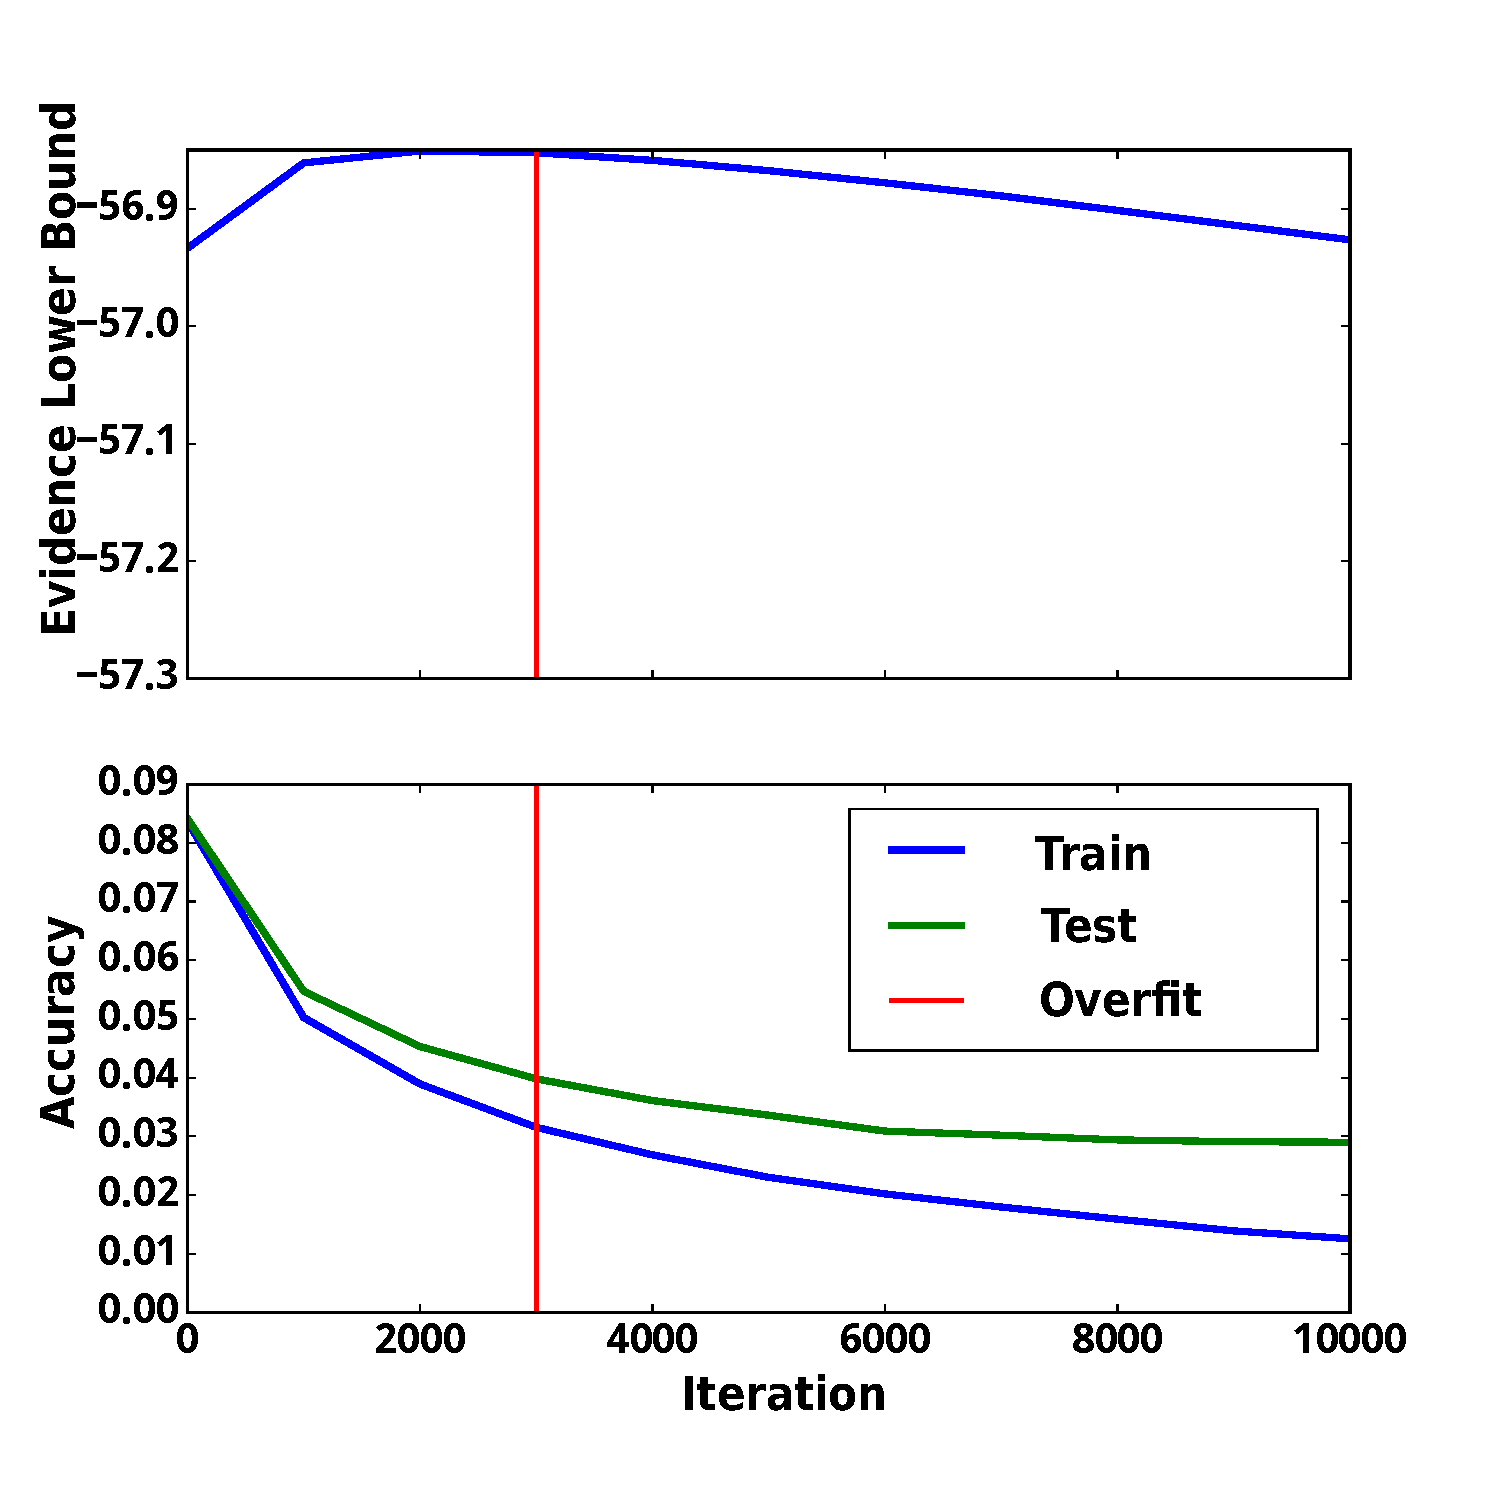
\includegraphics[width=0.4\textwidth]{./slide_plots/sgd_show_en.pdf}}
\end{figure}
\end{multicols}
\end{frame}





\begin{frame}{Model selection problem}
\footnotesize
Define a variational distribution $q=q_\mathbf{w}q_{\boldsymbol{\Gamma}}$ with parameters $\boldsymbol{\theta}$ that approximates posterior distribution $p(\mathbf{w}, \boldsymbol{\Gamma}|\mathbf{X}, \mathbf{y}, \mathbf{h}, \mathbf{f})$.



\begin{block}{Definition}

\textit{Loss function} $\Loss$ is a differentiable function interpreted as a performance of the model on the train dataset.~\\~\\
\textit{Validation function} $\Val$  is a differentiable function  interpreted as a general performance of the model.
\end{block}
\begin{block}{}
The \textit{model selection problem} $\mathbf{f}$ is a level optimization:

\[
	\mathbf{h}^{*} = \argmax_{\mathbf{h} \in \mathbb{H}} \Val[][][][\teta^{*}],
\]
where $\boldsymbol{\theta}^{*}$ is a solution for the following optimization:
\[
   \boldsymbol{\theta}^{*} = \argmax_{\boldsymbol{\theta} \in \mathbb{U}} \Loss.
\]
\end{block}


\end{frame}







\begin{frame}{Proposed optimization problem}

\footnotesize
\begin{columns}
\begin{column}{0.8\textwidth}
\begin{block}{Theorem [Bakhtreev, 2019]}
The following problem is generalizing:
\[
\mathbf{h}^{*} = \argmax_{\mathbf{h}} Q = 
\]
\[
= \textcolor{blue}{\lamLL\mathsf{E}_{\q[\teta^{*}]} \text{log}~{p(\mathbf{y} | \mathbf{X}, \mathbf{w},\boldsymbol{\Gamma}, \mathbf{h}, \lam)}}
 -\]
\vspace{-0.3cm}
\[- \textcolor{red}{^\text{prior}_\text{Q}\text{D}_{KL}\bigl(\q[\teta^{*}] || p(\mathbf{w}, \boldsymbol{\Gamma} |\mathbf{h}, \lam) \bigr)}  -\]
\vspace{-0.3cm}
\[
 - \textcolor{OliveGreen}{\sum_{p' \in \mathfrak{P}, \lambda \in \boldsymbol{\lambda}^\text{struct}_\text{Q}} \lambda\text{D}_{KL}(\priorG | p') + \text{log}p(\mathbf{h}|\lam)}, 
\]
where 
\[
\teta^{*} = \argmax_{\teta} L = 
\textcolor{blue}{\mathsf{E}_q \text{log}~{p(\mathbf{y} | \mathbf{X}, \mathbf{w}, \boldsymbol{\Gamma}, \mathbf{h}, \lam)}}
\]
\vspace{-0.3cm}
\[- \textcolor{red}{^\text{prior}_\text{L}\text{D}_{KL}\bigl( q^{*}(\mathbf{w}, \boldsymbol{\Gamma}) || p(\mathbf{w}, \boldsymbol{\Gamma} |\mathbf{h}, \lam) \bigr)}.
\]
\end{block}
%$\lambda^\text{likelihood}_\text{L}, \lambda^\text{prior}_\text{L}, \lambda^\text{prior}_\text{Q},  \boldsymbol{\lambda}_{\text{struct}}^Q, \lambda_{\text{temp}}$ и параметры распределений $\mathbf{P}$ --- метапараметры оптимизации.\\
The proposed optimization generalized different optimization problems: maximum likelihood and evidence lower bound optimization, model complexity increase and decrease, exhaustive structure search.
\end{column}
\begin{column}{0.2\textwidth}
\begin{figure}
\centering
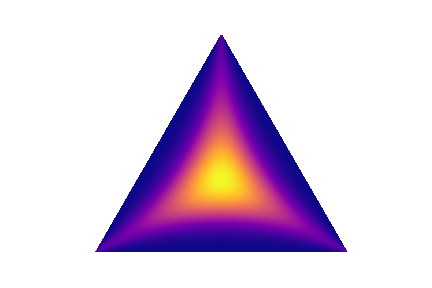
\includegraphics[width=0.75\textwidth]{combinations_1.png}
\end{figure}
\vspace{-0.2cm}
$ \textcolor{OliveGreen}{\boldsymbol{\lambda}_{\text{struct}}^Q=[0;0;0].}$
\begin{figure}
\centering
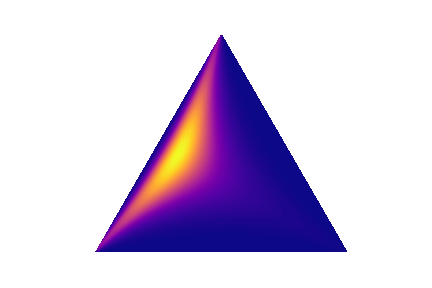
\includegraphics[width=0.75\textwidth]{combinations_2.png}
\end{figure}
\vspace{-0.2cm}
$ \textcolor{OliveGreen}{\boldsymbol{\lambda}_{\text{struct}}^Q=[1;0;0].}$
\begin{figure}
\centering
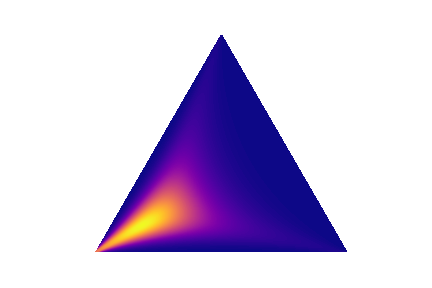
\includegraphics[width=0.75\textwidth]{combinations_3.png}
\end{figure}
\vspace{-0.2cm}
$ \textcolor{OliveGreen}{\boldsymbol{\lambda}_{\text{struct}}^Q=[1;1;0].}$
\end{column}
\end{columns}
\end{frame}









\begin{frame}{Hyperparameter optimization: example}
Toy example: polynomial regression with potential overfitting.\\

\begin{multicols}{2}

\begin{figure}[h]
\hspace*{-1cm}
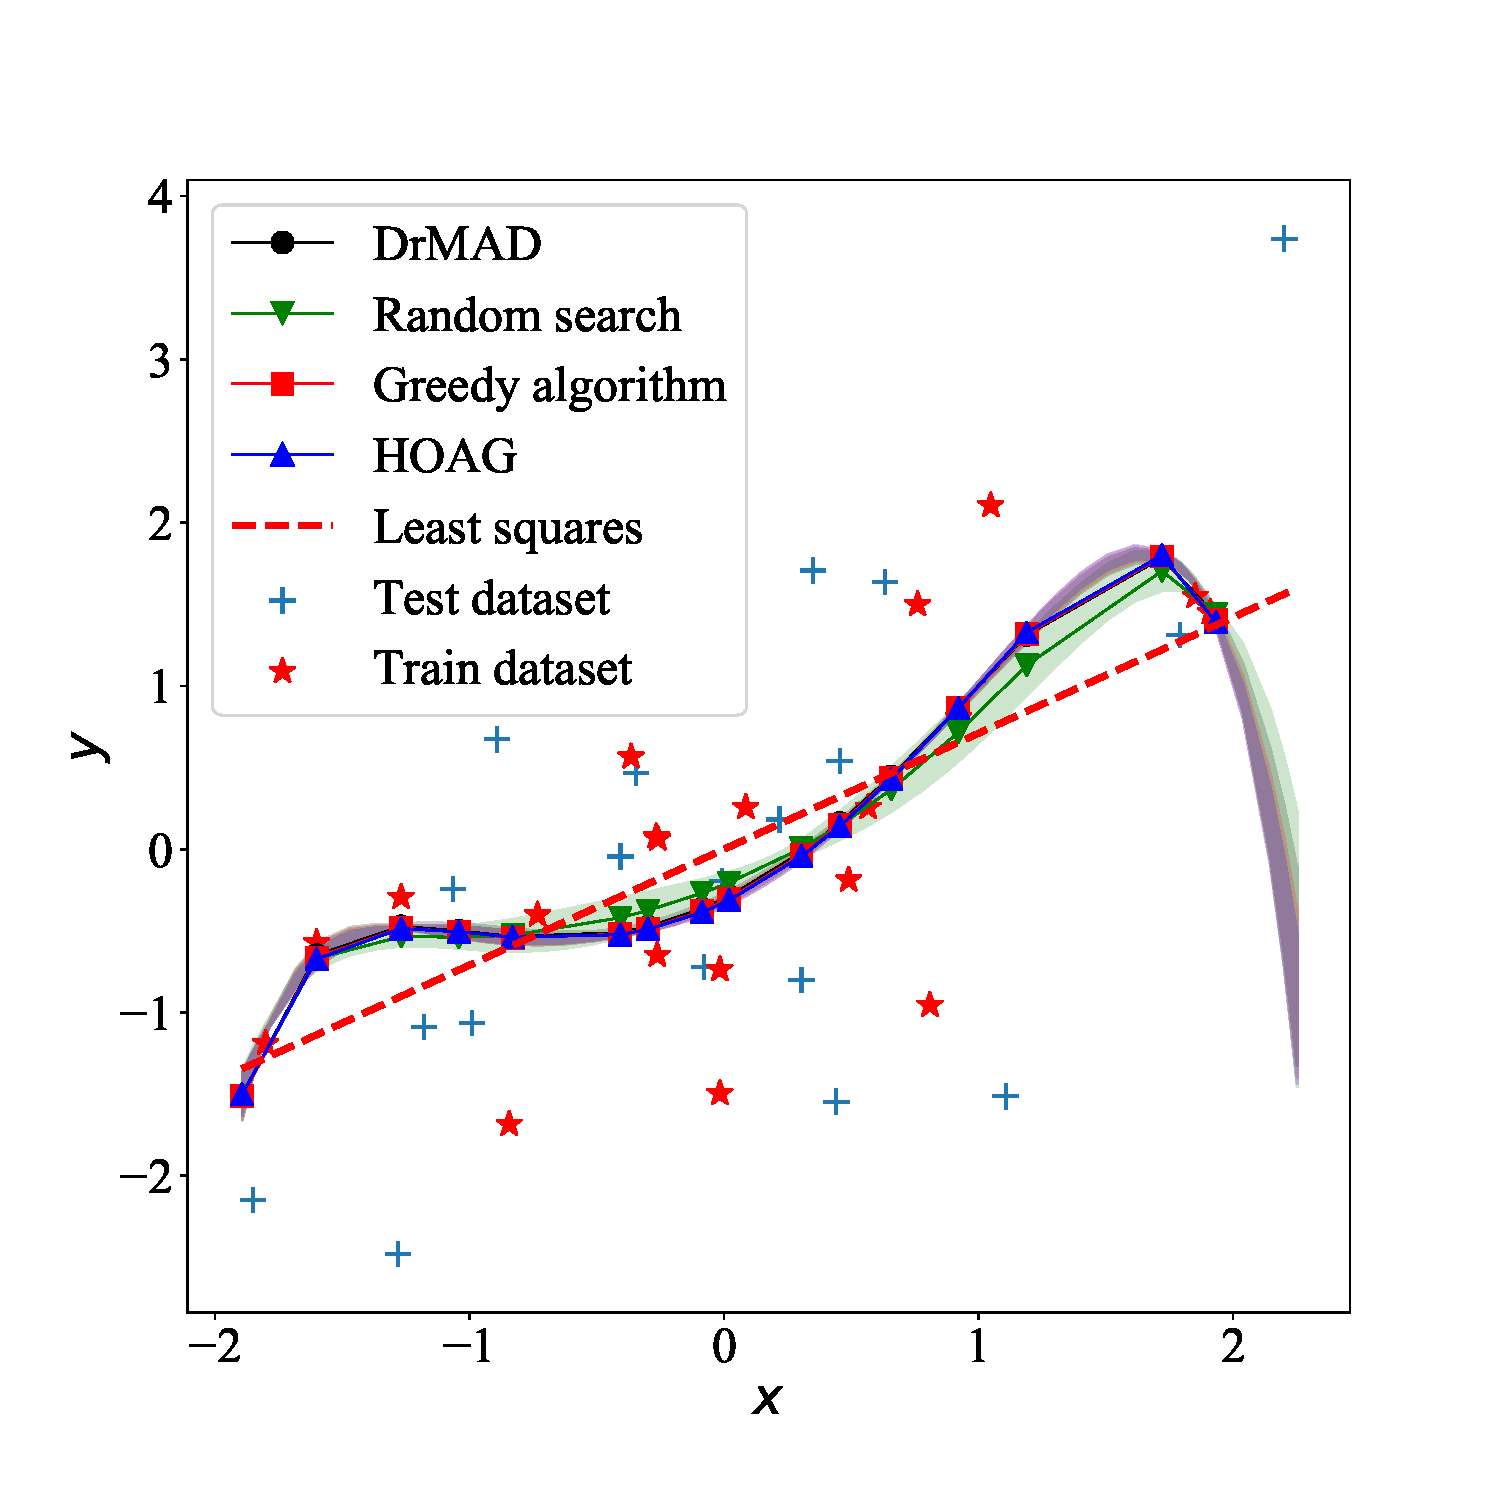
\includegraphics[width=0.5\textwidth]{./slide_plots/Fig_poly_cv2.pdf}
\caption*{Cross-validation}
\end{figure}

\begin{figure}[h]
\hspace*{-1cm}
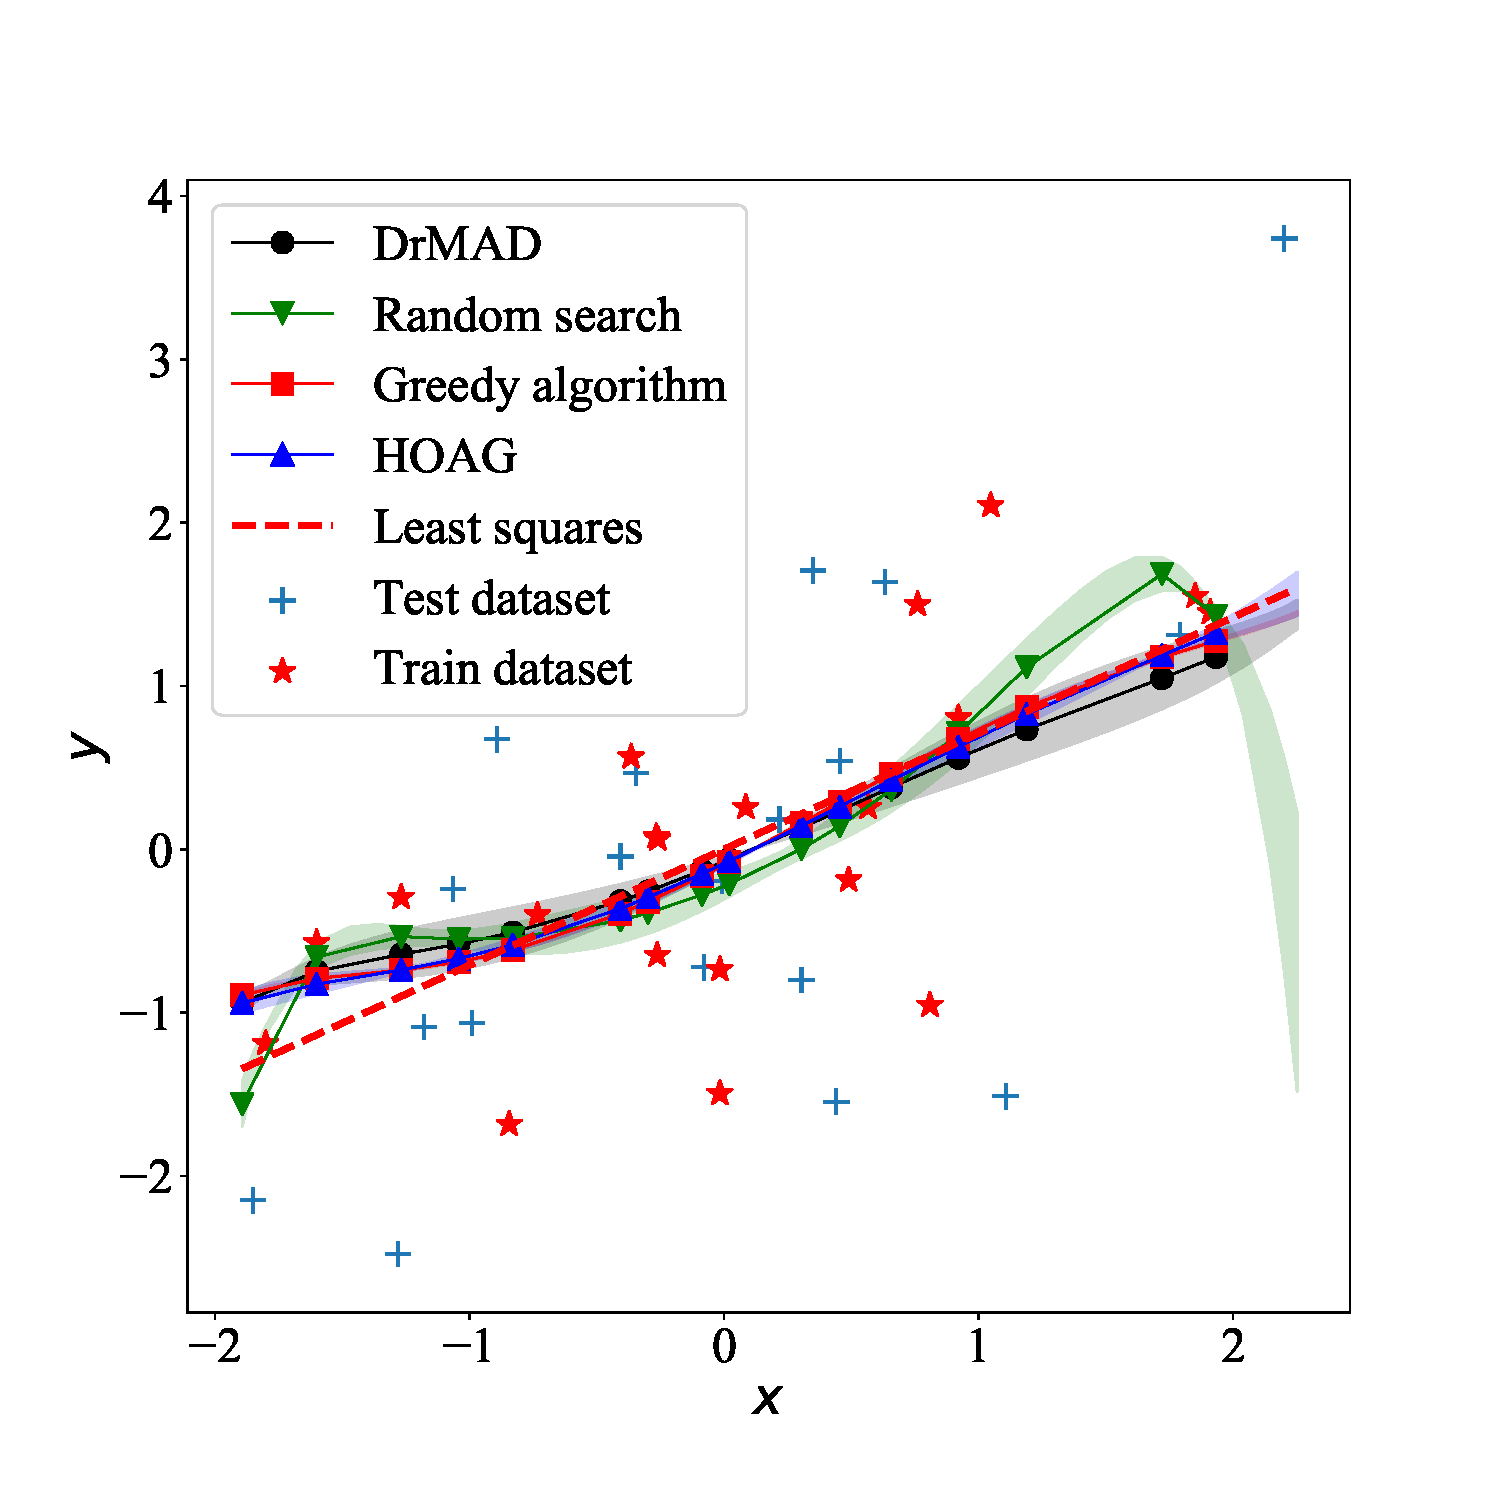
\includegraphics[width=0.5\textwidth]{./slide_plots/Fig_poly_var2.pdf}
\caption*{Evidence lower bound}
\end{figure}
\end{multicols}

\end{frame}




\begin{frame}{Experiments: WISDM}
\begin{figure}  
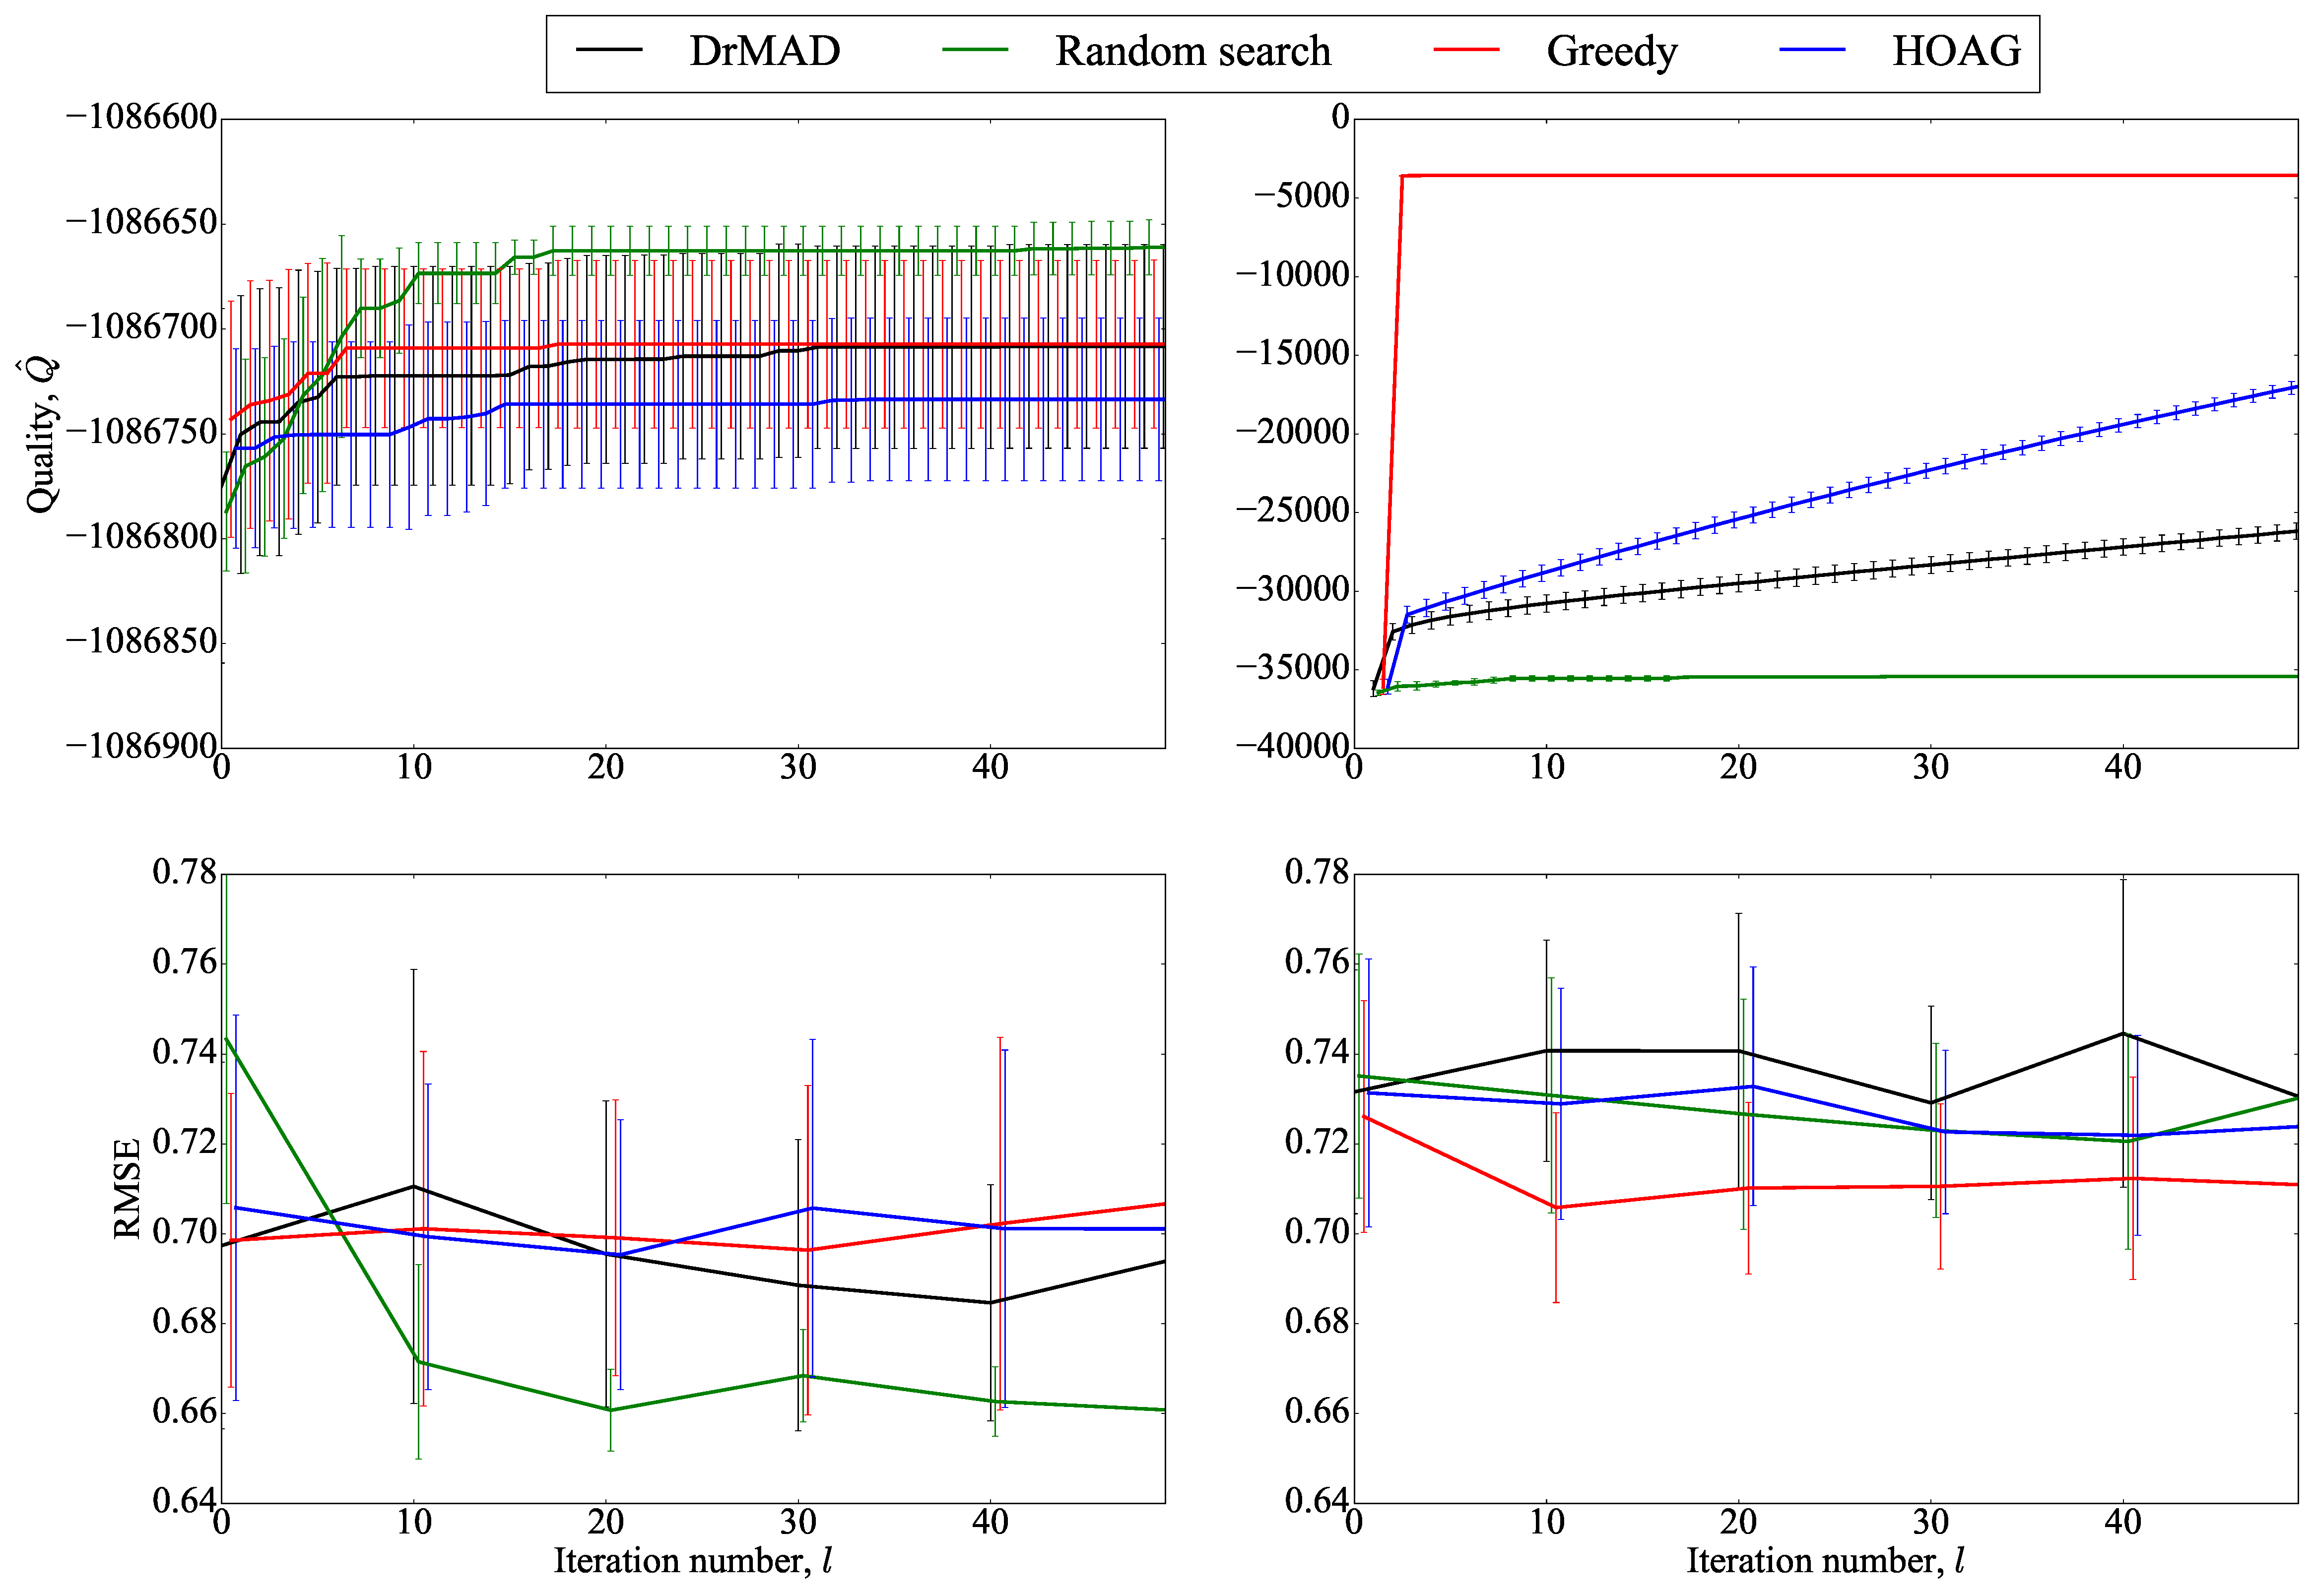
\includegraphics[width=0.75\textwidth]{Fig_wisdm.eps}
\end{figure}
\end{frame}










\begin{frame}[noframenumbering]
\frametitle{Toy example}
A model $\mathbf{f}$ is an ensebmle of 3 models:
\begin{enumerate}
\item $\mathbf{g}^{0,1}_0 = {tanh}(wx)$;
\item $\mathbf{g}^{0,1}_1 = {tanh}(\w^\mathsf{T} [x, x^2, \dots, x^{10}])$;
\item $\mathbf{g}^{0,1}_2 = {w}$.
\end{enumerate}

The optimization ran with three regimes:
\begin{itemize}
\item $\lambda_\text{prior} \ll \lambda_\text{likelihood}$; 
\item $\lambda_\text{prior} = \lambda_\text{likelihood}$;
\item $\lambda_\text{prior} \gg \lambda_\text{likelihood}$;
\end{itemize}


\end{frame}

\begin{frame}{Toy dataset: structures}

    \begin{table}
        \centering
        \begin{tabular}{cccc}

             & $\lambda_\text{temp}=0.2$ & $\lambda_\text{temp}=1.0$ & $\lambda_\text{temp}=10.0$  \\
          $\lambda_\text{prior} \ll \lambda_\text{likelihood}$    & 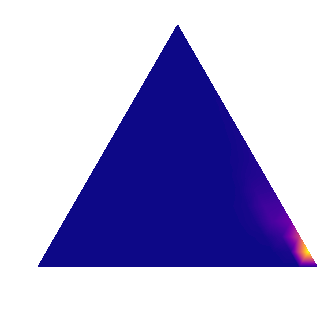
\includegraphics[width=0.15\textwidth]{triangle_0_2overfit.png} & 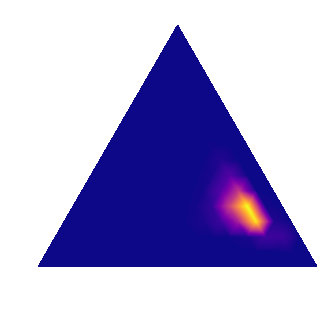
\includegraphics[width=0.15\textwidth]{triangle_1overfit.png} & 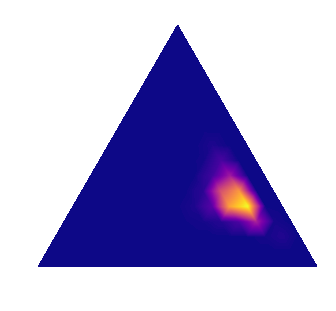
\includegraphics[width=0.15\textwidth]{triangle_10overfit.png}\\
         $\lambda_\text{prior} = \lambda_\text{likelihood}$    & 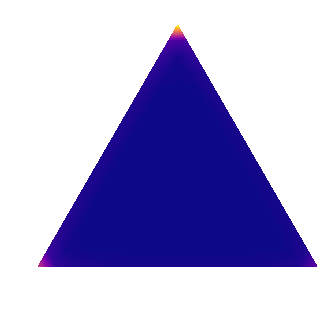
\includegraphics[width=0.15\textwidth]{triangle_0_2ok.png} & 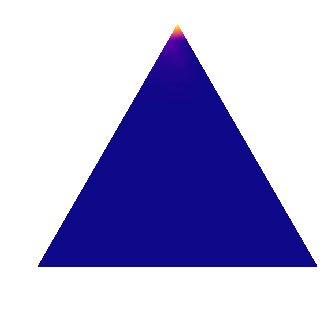
\includegraphics[width=0.15\textwidth]{triangle_1elbo.png} & 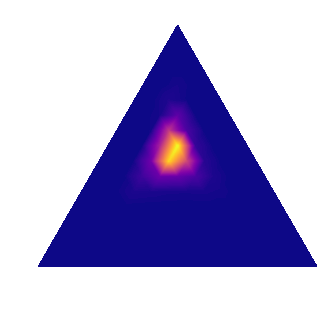
\includegraphics[width=0.15\textwidth]{triangle_10elbo.png}\\
          $\lambda_\text{prior} \gg \lambda_\text{likelihood}$   & 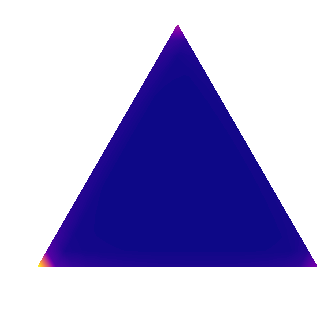
\includegraphics[width=0.15\textwidth]{triangle_0_2kld.png} & 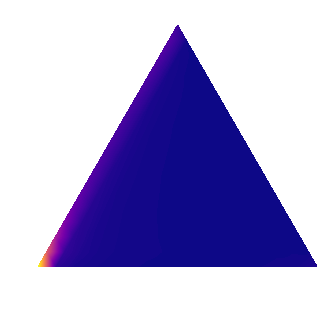
\includegraphics[width=0.15\textwidth]{triangle_1kld.png} & 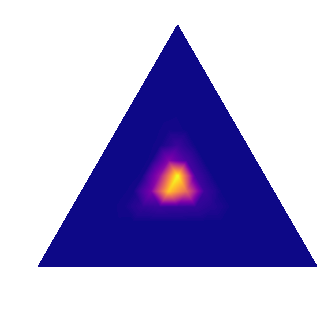
\includegraphics[width=0.15\textwidth]{triangle_10kld.png}\\
        \end{tabular}


    \end{table}
    
    
\end{frame}


\begin{frame}{Toy dataset: prediction performance}

    \begin{table}
        \centering
        \tiny
        \begin{tabular}{cccc}

             &  $\lambda_\text{temp}=0.2$ & $\lambda_\text{temp}=1.0$ & $\lambda_\text{temp}=10.0$  \\
          $\lambda_\text{prior} \ll \lambda_\text{likelihood}$    & 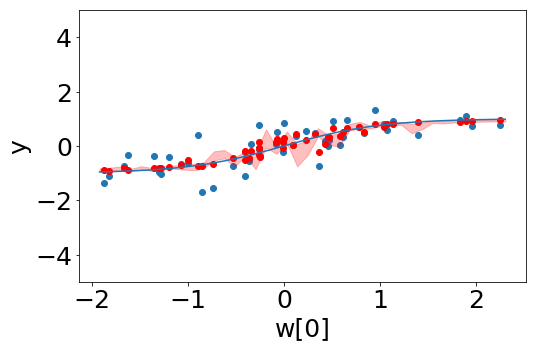
\includegraphics[width=0.25\textwidth]{plot_0_2overfit.png} & 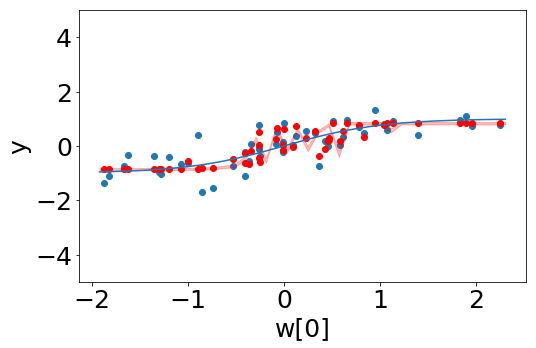
\includegraphics[width=0.25\textwidth]{plot_1overfit.png} & 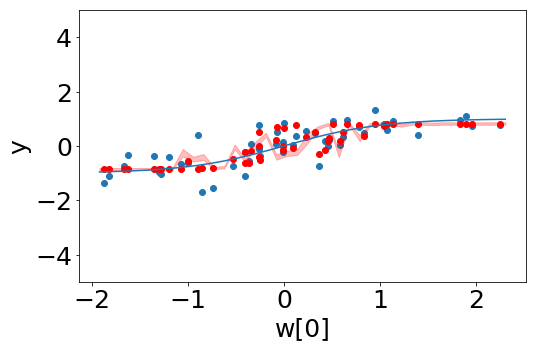
\includegraphics[width=0.25\textwidth]{plot_10overfit.png}\\
         $\lambda_\text{prior} = \lambda_\text{likelihood}$    & 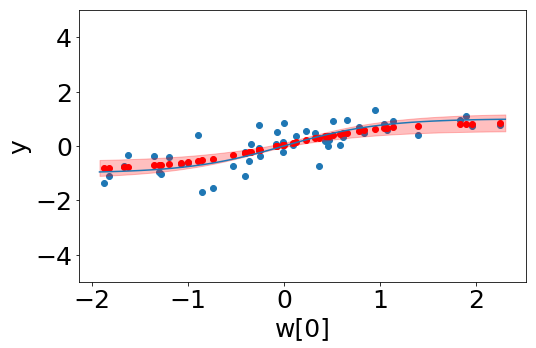
\includegraphics[width=0.25\textwidth]{plot_0_2ok.png} & 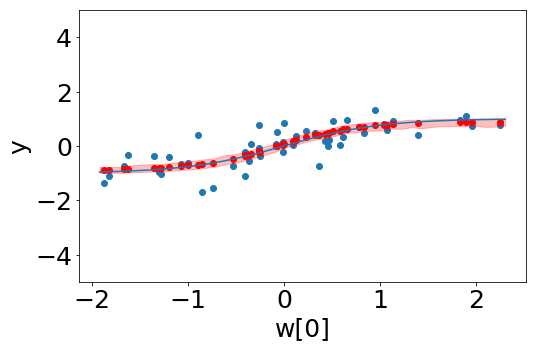
\includegraphics[width=0.25\textwidth]{plot_1elbo.png} & 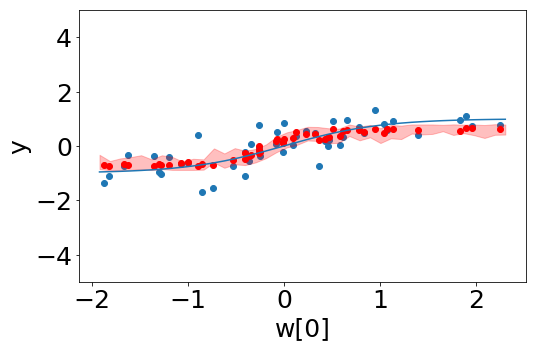
\includegraphics[width=0.25\textwidth]{plot_10elbo.png}\\
          $\lambda_\text{prior} \gg \lambda_\text{likelihood}$   & 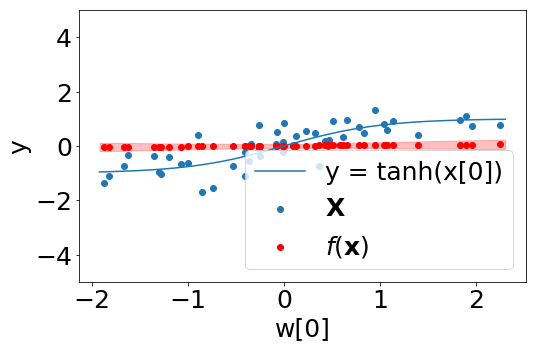
\includegraphics[width=0.25\textwidth]{plot_0_2kld.png} & 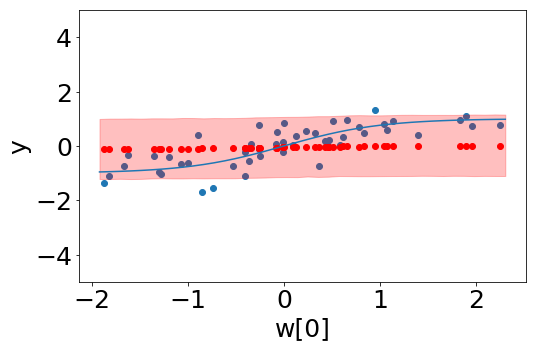
\includegraphics[width=0.25\textwidth]{plot_1kld.png} & 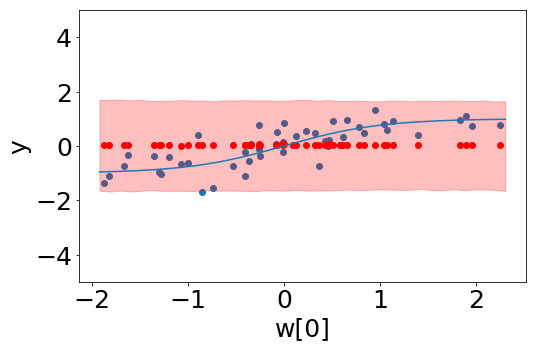
\includegraphics[width=0.25\textwidth]{plot_10kld.png}\\
        \end{tabular}

    \end{table}
    
    
\end{frame}



\begin{frame}{Example}
$\lambda_\text{prior}$ controls the importance of the prior distribution. With its increasing the model complexity decreases. 

\begin{figure}[h]
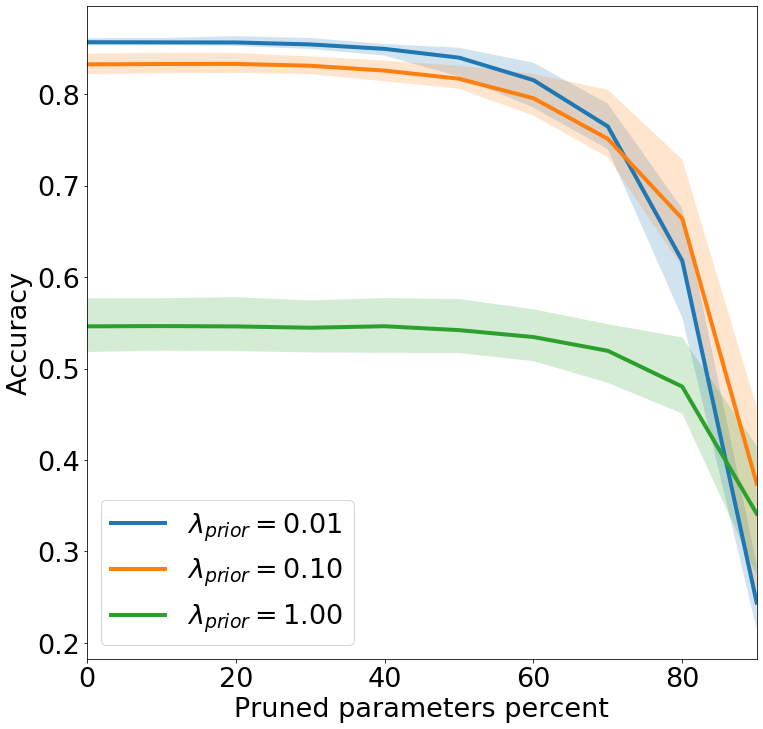
\includegraphics[width=0.4\textwidth]{./cifar_hyper.png}
\caption*{\footnotesize Grebenkova, Bakhteev, Strijov. Hypernetworks for deep model complexity control, 2021. (\textit{work in progress}).}
\end{figure}
\end{frame}


\begin{frame}{Current challenge}
\begin{itemize}
\item Can we control the model complexity at the inference step?
\item Can we select robust architrecture? What properties should it have?
\end{itemize}
\end{frame}

\begin{frame}{Model complexity control}
\begin{block}{Hypernetworks}
A hypernetwork is a mapping from a set of variables responsible for the properties of a desired model to a set of its parameters.
\end{block}

Optimize the model with hypernetworks in the following optimization procedure:
\[
\mathbb{E}_{\lambda \sim P(\lambda)}
(\log p(\mathfrak{D}| \mathbf{w(\lambda)})
- \lambda D_{\text{KL}}(q(\mathbf{w(\lambda)})||p(\mathbf{w})) 
\to \max.
\]

\begin{block}{Theorem, Grebenkova 2021}
The hypernetwork approximates not only deep learning model's performance, but also it's statistical propoerties.
\end{block}
\end{frame}


\begin{frame}{Example: CIFAR-10}
\vspace{-0.5cm}
\begin{multicols}{2}
\begin{figure}[h]
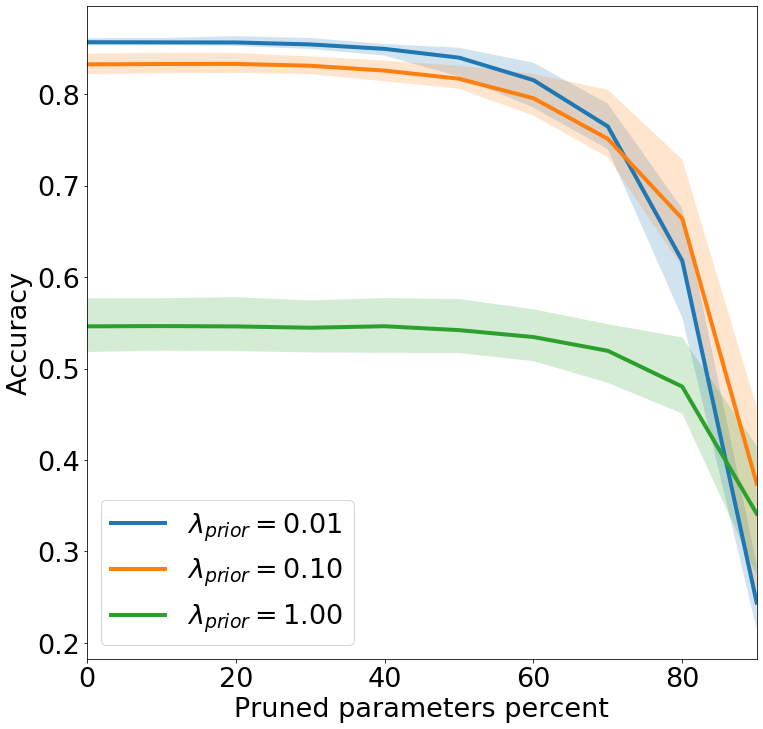
\includegraphics[width=0.4\textwidth]{./cifar_hyper.png}
\caption*{CNN}
\end{figure}

\begin{figure}[h]
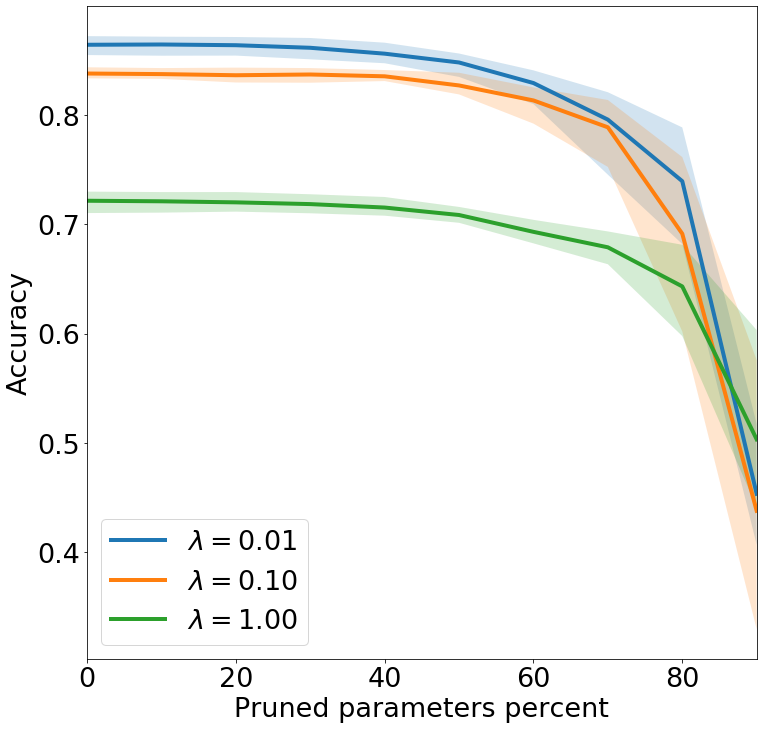
\includegraphics[width=0.4\textwidth]{./cifar_kernel.png}
\caption*{CNN with hypernetwork}
\end{figure}
\end{multicols}
{\footnotesize Grebenkova, Bakhteev, Strijov. Hypernetworks for deep model complexity control, 2021. (\textit{work in progress}).}
\end{frame}


\begin{frame}{Architecture complexity control}
\footnotesize
The hypernetworks can approximate not only the model parameter $\mathbf{w}$, but also structural parameters $\boldsymbol{\gamma}$.
\begin{block}{Baseline: DARTS}
A model architecture is a directed graph with non-linear operations $\mathbf{f}^{(i, j)}$ that are induced by basic functions $\mathbf{g}^{(i, j)}$ with weights obtained by softmax function application:
\[
\mathbf{f}^{(i, j)}(\mathbf{x}) = \langle \textbf{softmax}(\boldsymbol{\gamma}^{(i, j)}), {\mathbf{g}}^{(i,j)}(\mathbf{x})\rangle
\]
\end{block}

\begin{block}{Our proposal}
To use a mapping $\boldsymbol{\gamma}(\lambda_n)$ instead of constant structural parameters $\boldsymbol{\gamma}(\lambda_n)$, where $\lambda_n$ is a regularization term for the loss function:
\[
    \mathsf{E}_{\lambda_n} \left( \text{log}~p(\mathbf{y} | \mathbf{X}, \mathbf{w}, \boldsymbol{\Gamma}(\lambda_n))  +  \lambda_n \sum_{(i,j)}    \langle \textbf{softmax}\left( \frac{\boldsymbol{\gamma(\lambda_n)}^{(i, j)}}{\lambda_\text{temp}} \right), \mathbf{n}({\mathbf{g}}^{(i,j)})\rangle  \right),   
\]
where $\mathbf{n}({\mathbf{g}}^{(i,j)})$ is a vector of amount of parameters for all the basic functions $\mathbf{g}$.
\end{block}

\end{frame}


\begin{frame}{Example: Fashion-MNIST}
\begin{figure}[h]
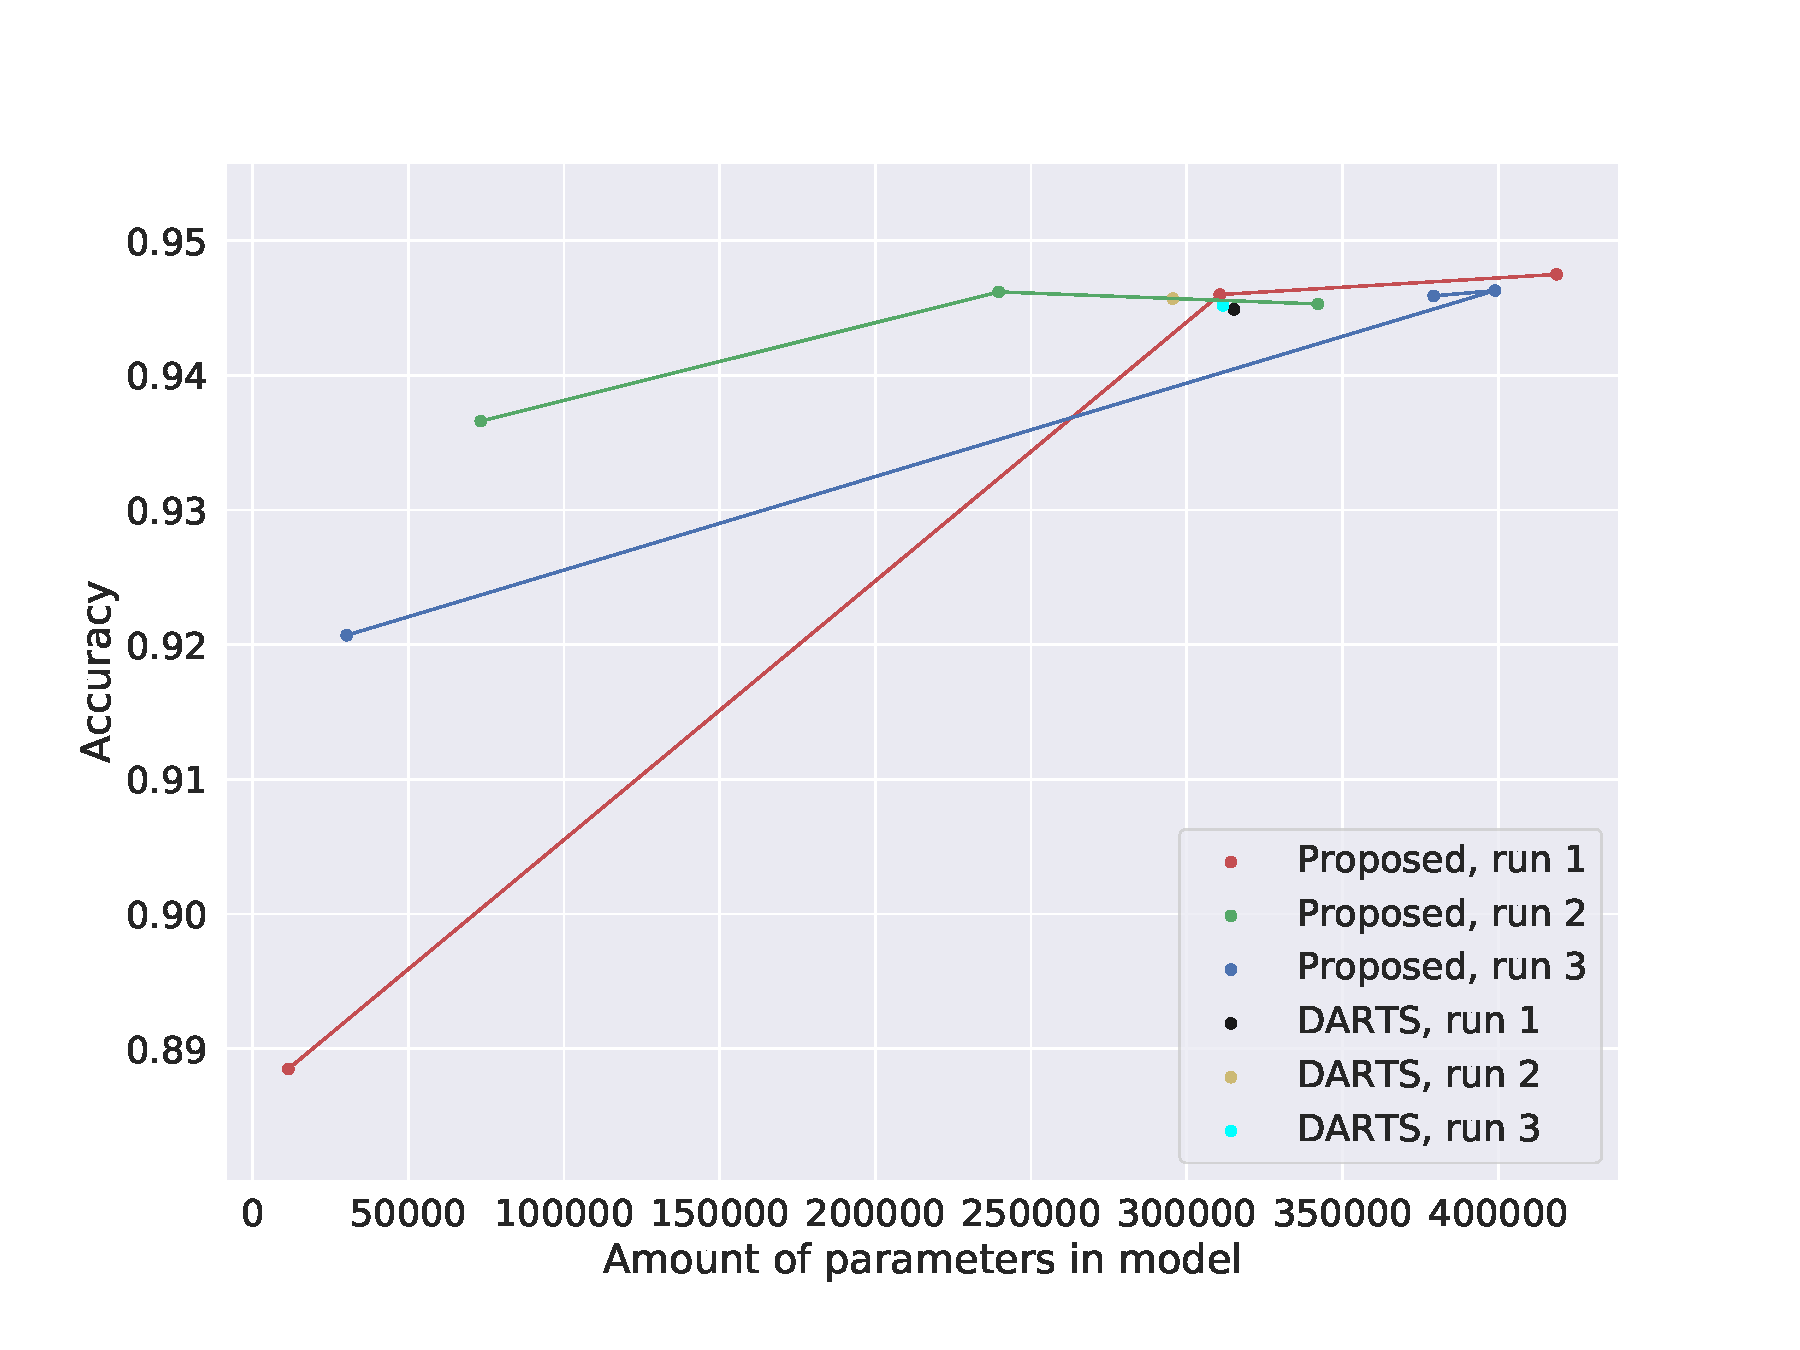
\includegraphics[width=0.6\textwidth]{./darts.pdf}
\caption*{\footnotesize Yakovlev, Grebenkova, Bakhteev, Strijov. Automated architecture search with model complexity control, 2021. (\textit{work in progress}).}
\end{figure}
\end{frame}


\begin{frame}{Example}
\vspace{-0.5cm}
\begin{multicols}{2}
\begin{figure}[h]
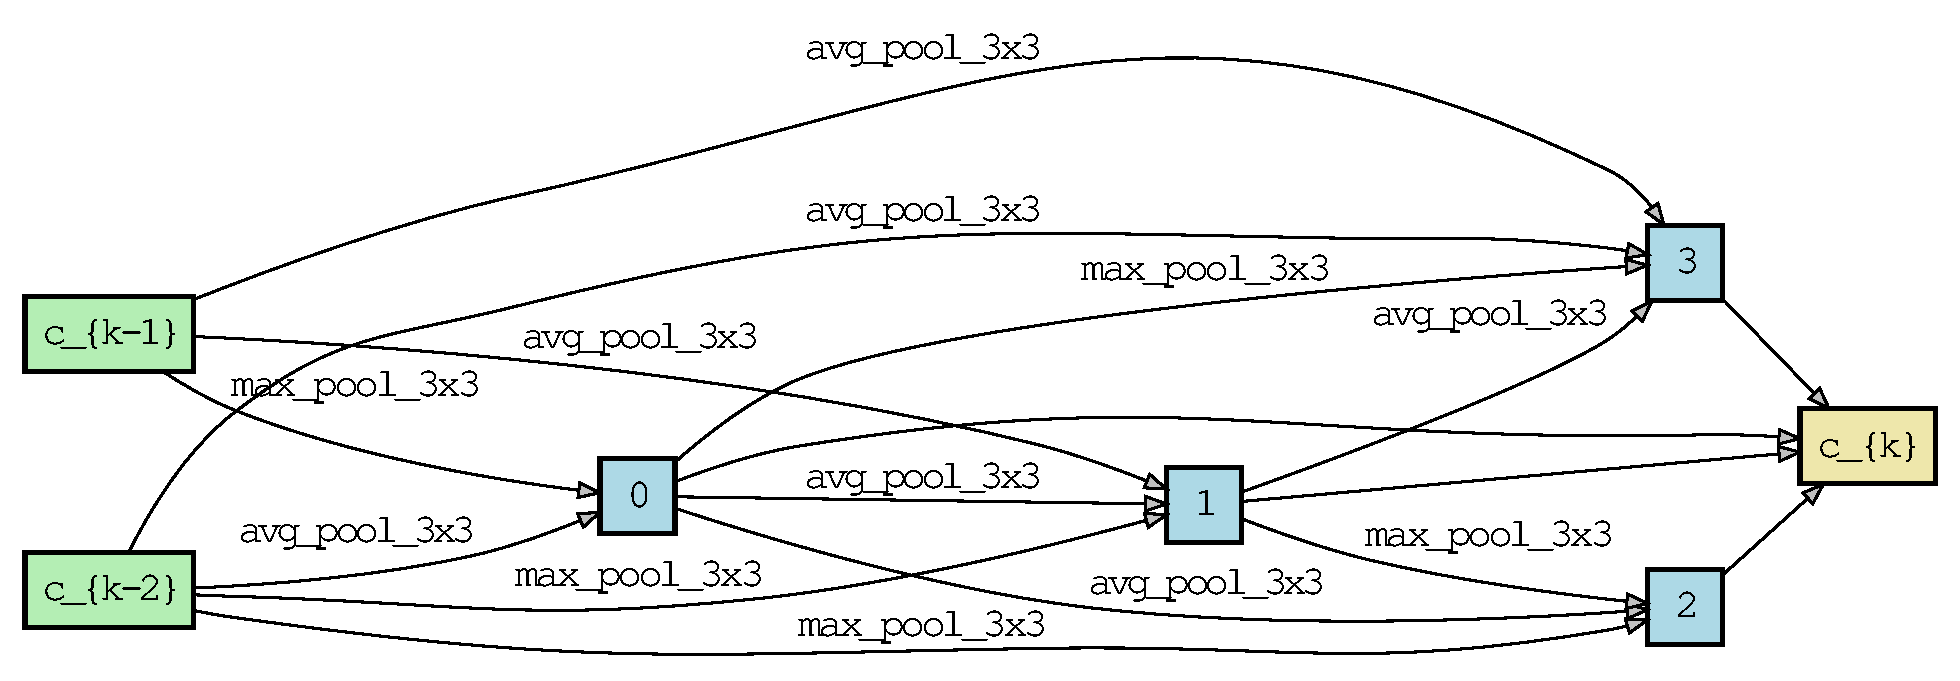
\includegraphics[width=0.45\textwidth]{./geno_2.eps}
\caption*{Simple CNN cell architecture}
\end{figure}

\begin{figure}[h]
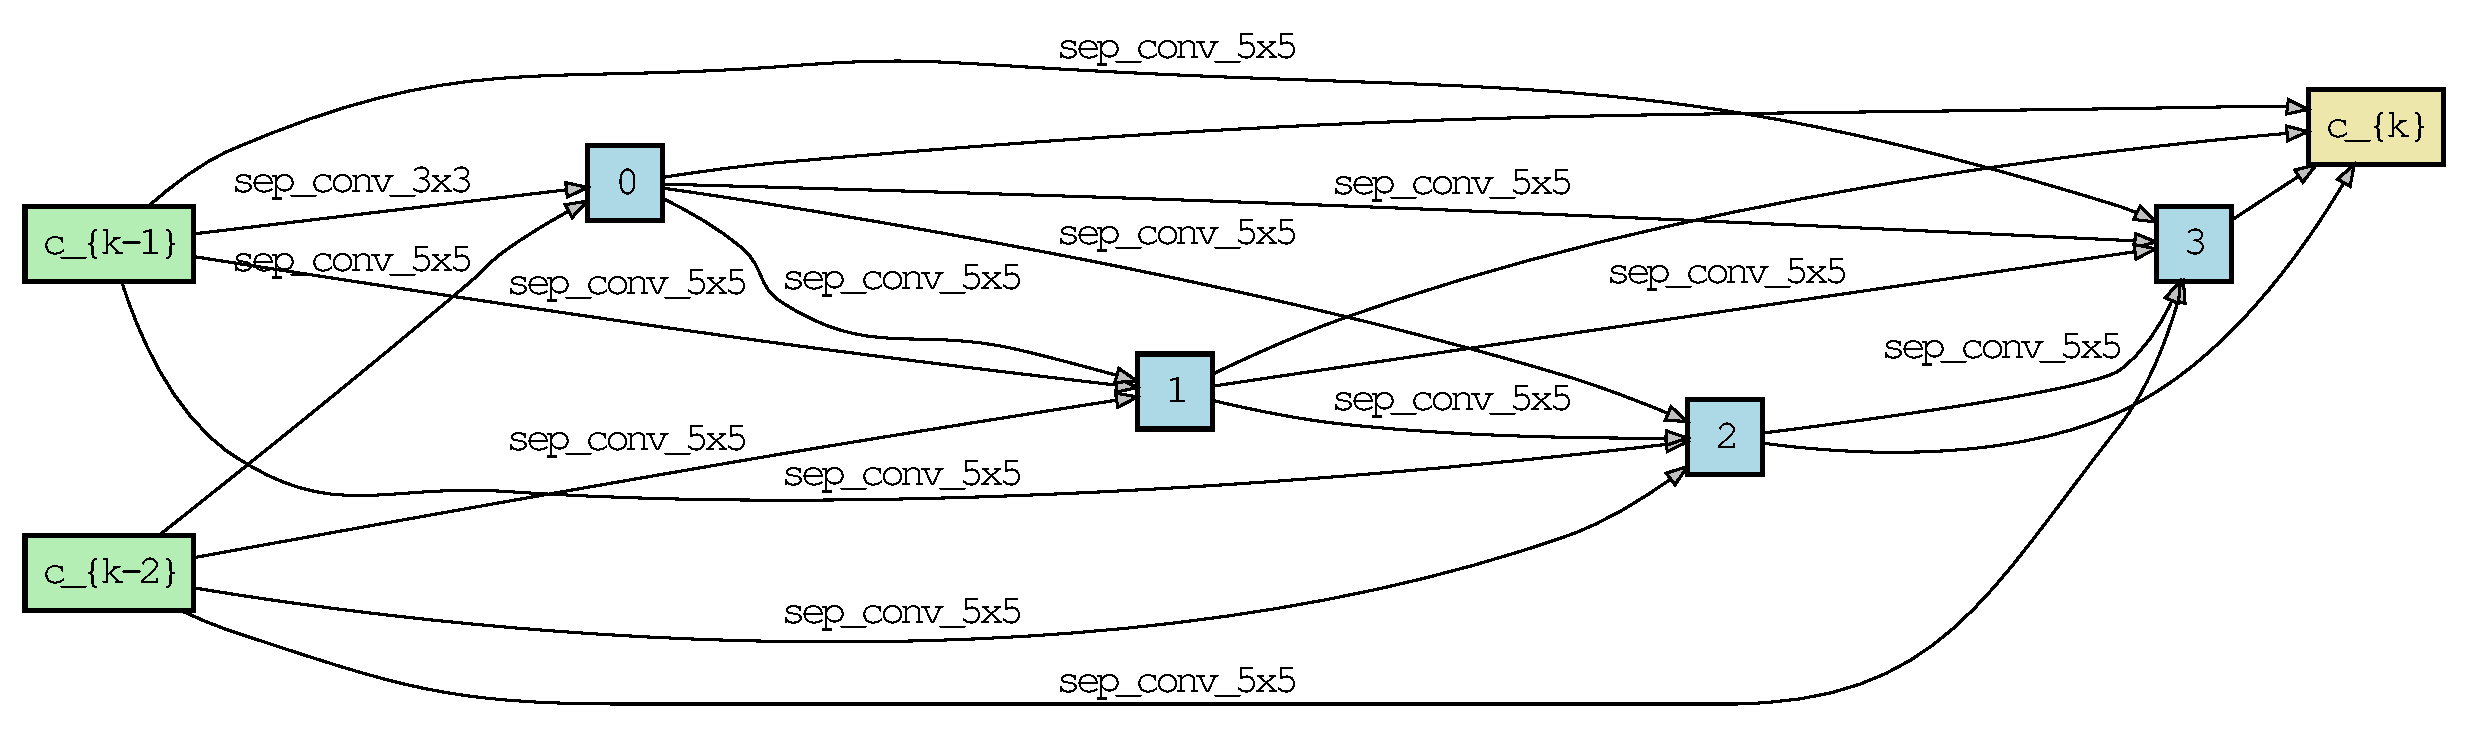
\includegraphics[width=0.45\textwidth]{./geno_1.eps}
\caption*{Complex CNN cell architeuctre}
\end{figure}
\end{multicols}
\vspace{-0.5cm}
{\footnotesize Yakovlev, Grebenkova, Bakhteev, Strijov. Automated architecture search with model complexity control, 2021. (\textit{work in progress}).}
\end{frame}
 




\begin{frame}{Robust architecture}
\begin{itemize}
\item Robustness to noise in data
\begin{itemize}
\item Random noise
\item Adversarial attacks
\end{itemize}
\item Robustness to model modification
\begin{itemize}
\item Parameters modification
\item Structure modification
\end{itemize}
\end{itemize}
\end{frame}





\begin{frame}{Experiments: MNIST}
Correct hyperparameter optimization leads to the model robustness under noise adjustment:  $\mathcal{N}(\mathbf{0},\sigma^2\mathbf{I})$.

\setlength{\columnsep}{10pt}
\begin{multicols}{4}
\begin{figure}[h]
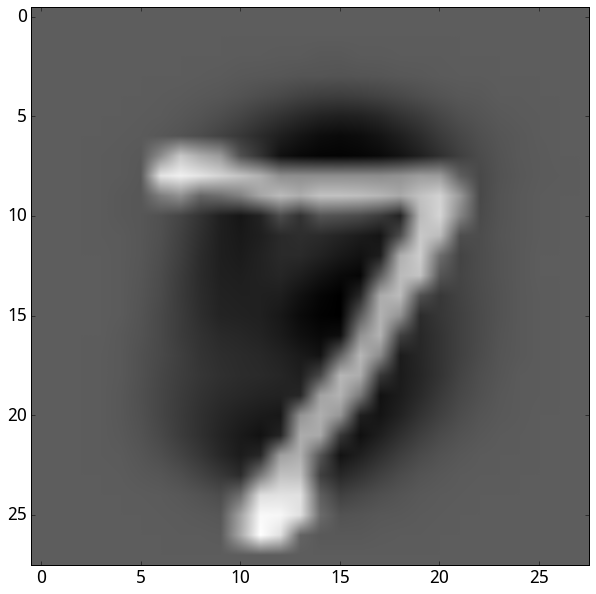
\includegraphics[width=0.10\textwidth]{./mnist0.png}
\caption*{Original images}
\end{figure}

\begin{figure}[h]
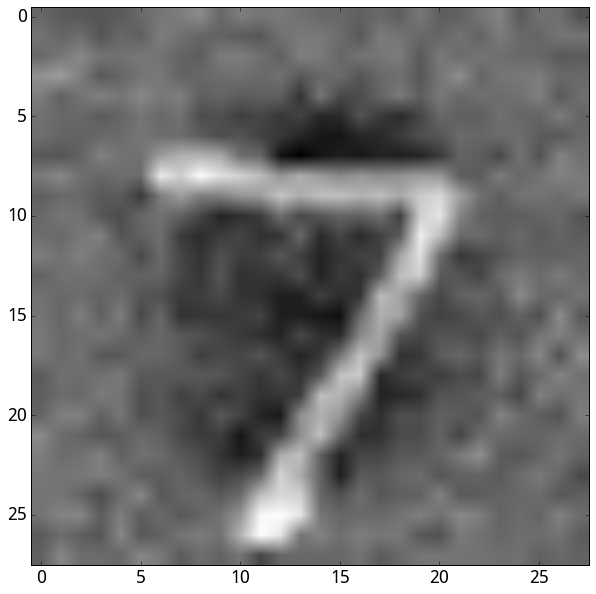
\includegraphics[width=0.08\textwidth]{./mnist10.png}
\caption*{$\sigma=0.1$}
\end{figure}

\begin{figure}[h]
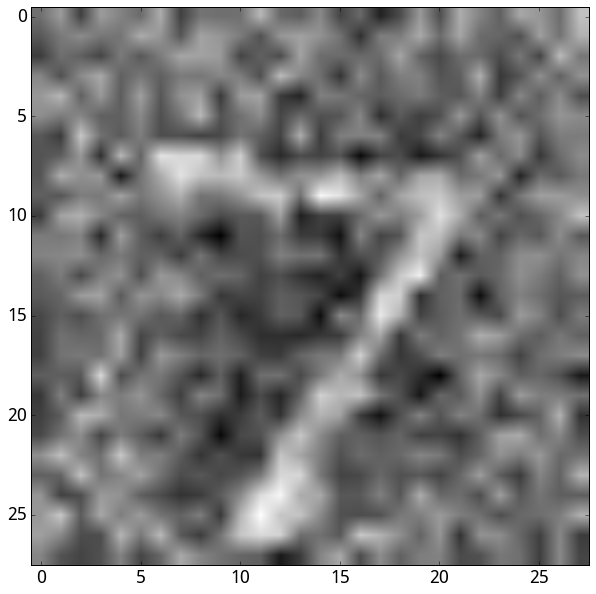
\includegraphics[width=0.08\textwidth]{./mnist25.png}
\caption*{$\sigma=0.25$}
\end{figure}

\begin{figure}[h]
\includegraphics[width=0.08\textwidth]{./mnist50.png}
\caption*{$\sigma=0.5$}
\end{figure}
\end{multicols}
\begin{center}
\includegraphics[width=0.85\textwidth]{Fig_noise.pdf}
\end{center}
\end{frame}



\begin{frame}{Robustness to adversarial attacks}
FGSM-method: $\hat{\mathbf{x}} = \mathbf{x} + \epsilon \cdot \textbf{sign}(\nabla_{\mathbf{x}} \log p(y|\mathbf{x}, \mathbf{w}, \boldsymbol{\Gamma}, \mathbf{f})).$

\begin{figure}[h]
\includegraphics[width=0.6\textwidth]{./var_fgm.png}
\caption*{Simple CNN cell architecture}
\end{figure}

\end{frame}


\begin{frame}{Robustness to struccture pruning}

\begin{figure}[h]
\includegraphics[width=0.6\textwidth]{./var_struct.png}
\caption*{Simple CNN cell architecture}
\end{figure}

\end{frame}


\begin{frame}{References}
\end{frame}

\end{document}
